%%%%%%%%%%%%%%%%%%%%%%%%%%%%%%%%%%%%%%%%%%%%%%%%%%%%%%%%%%%%%%%%%%%%%%%%%%%%%%%%
%2345678901234567890123456789012345678901234567890123456789012345678901234567890
%        1         2         3         4         5         6         7         8

%\documentclass[preprint,5p]{elsarticle}
\documentclass[preprint,3p,times]{elsarticle}

\usepackage[utf8x]{inputenc}
\usepackage[T1]{fontenc}

\usepackage[english]{babel}
\usepackage{graphicx, subfigure}

\usepackage[draft,nomargin, marginclue, footnote]{fixme}

\newcommand{\concept}[1]{{\small \texttt{#1}}}
\newcommand{\stmt}[1]{{\footnotesize \tt $\langle$ #1\relax$\rangle$}}

\newcommand{\ie}{{\textit{i.e.\ }}}
\newcommand{\cf}{{\textit{cf\ }}}
\newcommand{\eg}{{\textit{e.g.\ }}}
\newcommand{\al}{{\textit{et al.\ }}}

\graphicspath{{figs/}}
\DeclareGraphicsExtensions{.pdf,.jpg,.png}

\begin{document}
\begin{frontmatter}

\title{\LARGE \bf
Human-Robot Interaction: Tackling the AI Challenges
}

\author{Séverin Lemaignan, Mathieu Warnier, E. Akin Sisbot, Rachid Alami}

\address{
CNRS, LAAS, 7 avenue du Colonel Roche, F-31400 Toulouse, France\\
Univ de Toulouse, LAAS, F-31400 Toulouse, France\\
{\tt firstname.lastname@laas.fr}
}




%%%%%%%%%%%%%%%%%%%%%%%%%%%%%%%%%%%%%%%%%%%%%%%%%%%%%%%%%%%%%%%%%%%%%%%%%%%%%%%%
\begin{abstract}

Human-Robot interaction is an area filled with challenges for artificial
intelligence: dynamic, partially unknown environments that are not originally
designed for autonomous machines; a large variety of situations and objects to
deal with, with possibly complex semantics; physical interactions with humans
that requires fine, low-latency control, representation and management of
several mental models, good situation assessment skills...the list goes on.

This article sheds light on some key decisional issues that are to be tackled
for a cognitive robot to share space and tasks with a human, and present our
take on these challenges. We adopt a constructive approach based on the
identification and the effective implementation of individual and collaborative
skills. These cognitive abilities cover geometric reasoning and situation
assessment mainly based on perspective-taking and affordances, management and
exploitation of each agent (human and robot) knowledge in separate cognitive
models, natural multi-modal communication, human-aware task planning, and human
and robot interleaved plan achievement.

We present our design choices, the articulations between the diverse
deliberative components of the robot, experimental results, and eventually
discuss the strengths and weaknesses of our approach. It appears that
\emph{explicit} knowledge management, both symbolic and geometric, proves to be
key as it pushes for a different, more \emph{semantic} way to address the
decision-making issue in human-robot interactions.

\end{abstract}

\begin{keyword}
    %% keywords here, in the form: keyword \sep keyword
    human-robot interaction \sep cognitive robotics \sep perspective taking \sep knowledge representation and reasoning
    %% MSC codes here, in the form: \MSC code \sep code
    %% or \MSC[2008] code \sep code (2000 is the default)

\end{keyword}

\end{frontmatter}

%%%%%%%%%%%%%%%%%%%%%%%%%%%%%%%%%%%%%%%%%%%%%%%%%%%%%%%%%%%%%%%%%%%%%%%%%%%%%%%%

\section{The challenge of human-robot interaction}

Human-robot interaction is a challenge for artificial intelligence. This field
indeed lays at the crossroad of several other domains of AI and requires to
tackle them in a holistic manner: Modeling humans and human cognition;
acquiring, representing, manipulating in a tractable way abstract knowledge;
reasoning on this knowledge to make decisions; and eventually instantiating
those decisions into physical actions in coordination with humans. Many AI
techniques are invited, from visual processing to symbolic reasoning, from task
planing to \emph{theory of mind} building, from reactive control to action
recognition and learning.

We do not tackle all these issues. This article attempts however to organize
them into a coherent challenge for artificial intelligence, and also explicit
some of the paths that have been investigated on our robots and that result in a
deliberative, knowledge-oriented, architecture for human-robot interaction.


We scope our work to the robot which is
expected to achieve interactive object manipulation, fetch and carry tasks and
similar tasks in a domestic environment (Figure~\ref{fig:hri-dec}).

Two agents (a human and a robot) share a common space and exchange information
through multiple modalities. The robot is expected to explicitly take into
account the human and to manage its interactions with him.

Namely, the robot must be able to recognize, understand and participate
to communication situations, both explicit (\eg the human addresses verbally
the robot) and implicit (\eg the human points to an object); the robot must be
able to take part to joint actions, both proactively (by planning and proposing
such an action to the human) and reactively; the robot must be able to move and
act in a safe, efficient and legible way, taking into account social rules like
proxemics.

\begin{figure}[htb]
\centering
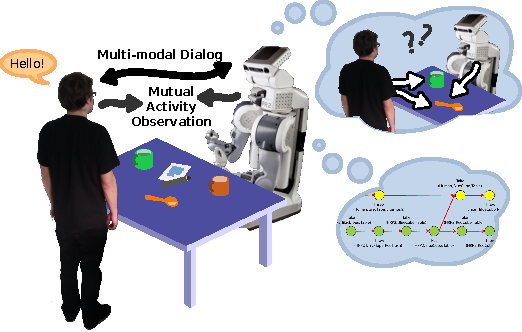
\includegraphics[width=0.9\columnwidth]{grounding_robot.pdf}
\caption{Robot reasoning about HRI and anticipation of human activities.
  Sources of information are multi-modal dialogue, and monitoring of the
  environment and human activity. The robot must adapt on-line its behaviours
  by merging computed plans with reactive control.}
\label{fig:hri-dec}
\end{figure}

Those three items have broad implications regarding the required underlying
cognitive skills.  A \emph{joint action}, for instance, can be described as
follow. Given:

\begin {itemize}
\item a joint goal, which has been previously established and agreed
  upon (typically through dialogue),
\item the current situation, acquired through perception or
  deduction from previous perceptions, including the state of the
  environment of the robot and of the human,
\item {\it a priori} common-sense knowledge,
\end {itemize}

the robot controller computes an action to execute and who (the 
human or the robot, or both in case of a joint action) has to perform
it, and then controls or monitors its execution. The operation
continues until the goal is achieved, is declared unachievable or is
abandoned by the human.

To do so, the robot has to be equipped with a number of decisional, planning
and interpretation abilities where its human partner is taken explicitly into
account. It needs to be able:

\begin{itemize}
\item to build and maintain relevant robot and human beliefs
  (from the robot perspective) with respect to state of the world and the task,
\item to build and maintain iteratively shared (human-robot) plans, 
\item to refine and execute the actions it has to perform, and to monitor 
those achieved by its human partner.
\end{itemize}

Besides, we would like to build such abilities in a generic way, and
to provide several levels of parametrization allowing to adapt to
various environments, and various levels of involvement of the robot
ranging from teammate behavior to assistant or proactive helper.

We will see, in the following sections, how cognitive skills for realistic
human-robot interaction can be implemented and organized together in a coherent
architecture.

\subsection{Article organization}

The remaining of the article discuss the robotic architecture we have built to
tackle the AI challenges of human-robot interaction, and how its relates to
other approaches. We propose to organize this discussion in four sections.

The next section presents the overall architecture and the knowledge model we
have developed for our robots. Section~\ref{sec:impl} gives some insights on
the each of the main components of the architecture, and try to highlight their
significance for artificial intelligence. Section~\ref{sec:expe} presents two
experiments that illustrate in a concrete way what can be currently achieved
with our robots.  Section~\ref{sect|conclusion} finally summarizes our main
contributions and relate them to other recent researches in the field.

\section{From human-robot interaction to a deliberative architecture}

\subsection{Building a human-aware deliberative layer}

\fxwarning{Need to carefully introduce this section: how did we come up this this architecture? Describe archi}

Over the last years, we have been slowly ramping up explicit knowledge
representation and manipulation in the deliberative and executive layers of our
robots. Ranging from situation assessment to symbolic task planning, from
verbal interaction to event-driven execution control, we have built up a
\emph{knowledge-oriented} architecture which is now used on a daily basis on
our robots.


Figure~\ref{fig|archi} gives an overview of the connections between the
deliberative components of our architecture~\cite{Alami2011}.

\begin{figure*}
        \centering
        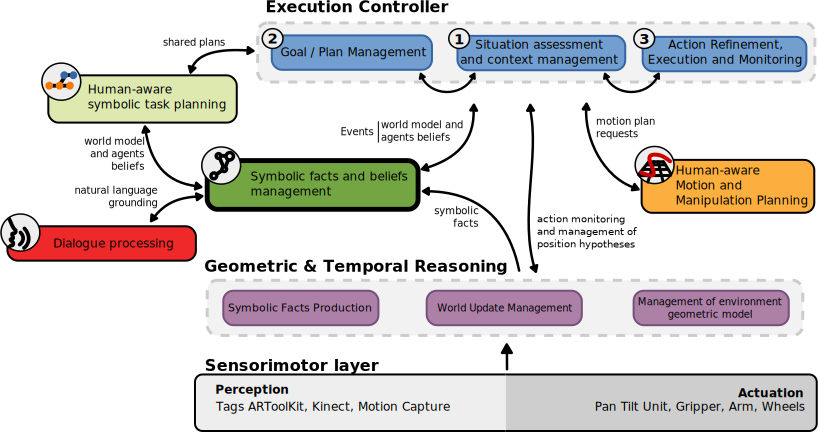
\includegraphics[width=0.8\textwidth]{archi}
        \caption{Overview of the LAAS deliberative layer. Knowledge is
        centrally managed in an active \emph{semantic blackboard}, pictured
        above with a thick border.}
        \label{fig|archi}
\end{figure*}


This architecture moves away from standard layered approaches found in
robotics~\cite{Gat1998three, Volpe2001CLARAty, Goldberg2002}. Interactions
between components at the deliberative level are mostly bidirectional and we do
not introduce layers of abstraction amongst software components\footnote{We do
have lower-level modules to execute actions or manage sensors, but all
cognition-related modules reside at the same level.}. Dialogue processing, for
instance, illustrates this structure: This component does not simply act as an
alternative perceptual input to the symbolic database; it also
actively queries previously acquired knowledge to disambiguate and validate the
newly created symbolic knowledge (see section~\ref{sect|com}).

Our architecture relates to \emph{Beliefs, Desires, Intentions} (BDI)
architectures. BDI architectures are primarily focused on \emph{practical
reasoning}, \ie the process of deciding, step by step, which action to perform
to reach a goal (as summarized by Woolridge~\cite{Woolridge1999}). The
management of the interaction between knowledge (the beliefs) and task and plan
representation and execution (the desires and the intentions) is central, and
aims at selecting at each step the best subgoal. It becomes then an intention
that the robot commits to.

This interaction between knowledge and actions is also central to our approach
(as for any cognitive system): it is one amongst all the activities carried by
the robot, actually performed by the communication components (that acquire
desires from interaction with agents) and the execution controller that may
decide to take an incoming desire into account to create its own internal
goals. The controller generates and manages intentions from these goals with
the help of a symbolic task planner, that also has direct access to the
knowledge base.

This activity is however not the backbone of our architecture. Other
activities are conducted in parallel, without being explicitly considered as
desires: assessment of the situation and the environment, dialogue (including
performative dialogue that can possibly change the internal state of the robot,
but does not lead to the creation of desires, like statement assertion or
question answering), various background monitoring and recognition tasks, etc.

Regarding the anchoring question, this architecture is bidirectional. The
components we described provide a \textit{bottom-up} grounding process:
geometric reasoning and dialogue processing modules constantly build and push
new symbolic contents about the world to the knowledge base where it becomes
accessible to decisional layers. In parallel, the knowledge base relies on
reasoning in a \textit{top-down} way to produce new facts that may in return
trigger physical behaviours.

\subsection{A Knowledge model}

In this architecture, knowledge manipulation relies on a
semantic \emph{blackboard}: a central server (the {\sc Oro}
server~\cite{Lemaignan2010}) stores knowledge as it is produced by each of the
deliberative components. It conversely exposes a {\tt json}-based RPC
API~\cite{lemaignan2012kbapi} to query the knowledge base.

Knowledge is represented as RDF triples in the OWL sub-language. Each
time triples are added or removed from the knowledge base, a Description
Logics reasoner ({\sc Pellet}\footnote{\tt http://clarkparsia.com/pellet/})
classifies the whole ontology and inserts all possible inferred triples.

At any time, the knowledge available to the robot may come from three sources:
{\it a priori} knowledge is stored in an ontology (the {\sc OpenRobots Ontology}),
loaded when the robot initializes. This static source covers the
\emph{common-sense} knowledge of the robot, and optionally some
scenario-specific knowledge (for instance about objects that are to be
manipulated). The second part of the knowledge is acquired at runtime from
perception, interaction, decision making.  We go over the processes it involves
in the next sections. Lastly, the third source of knowledge is the output of the
reasoner.

\begin{figure}
    \centering
    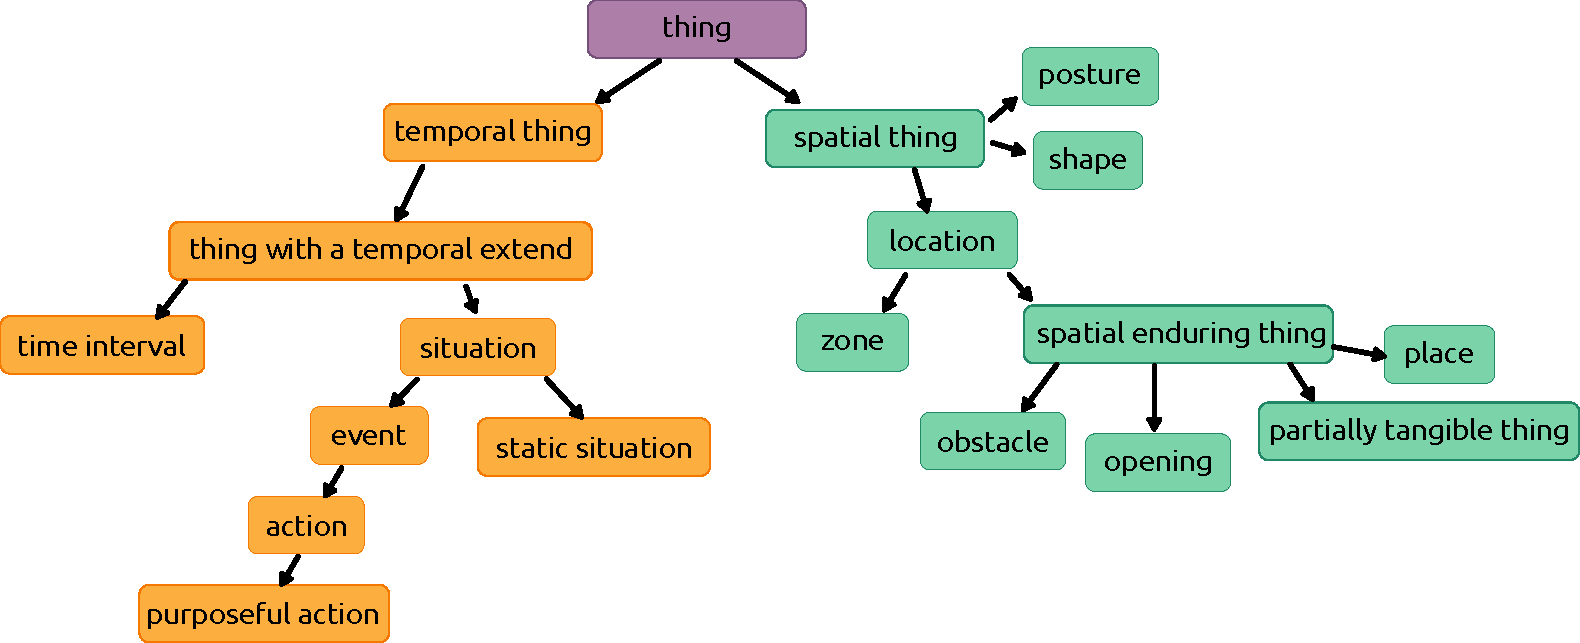
\includegraphics[width=\columnwidth]{top_tbox.pdf}

    \caption{The upper part of the ORO common-sense TBox. All these concepts
    belong to the {\sc OpenCyc} namespace.}
    
    \label{fig|upper_tbox}
\end{figure}

\paragraph{The OpenRobots Ontology} The ORO common-sense ontology has been designed from two requirements: covering
our experimental needs and conforming as much as possible to the {\sc OpenCyc}
upper ontology.

This lead to a bidirectional design process: from \emph{bottom-up} regarding
the choices of concepts to model, \emph{top-down} regarding the upper part of the
taxonomy. This upper part of the ontology is pictured on
Figure~\ref{fig|upper_tbox}. All the classes visible on this figure belong to the
{\sc OpenCyc} namespace (the {\tt cyc:} prefix is omitted for clarity).

Aligning the upper part of the ontology on {\sc OpenCyc} (as done by other
KRS, like {\sc KnowRob}~\cite{Tenorth2009a} or PEIS K\&R~\cite{Daoutis2009})
has multiple advantages. First the design of this part of the ontology is
generally difficult: it pertains to abstract concepts whose mutual relations
comes to philosophical debates. The upper taxonomy of {\sc OpenCyc} represents
a relative consensus, at least within the semantic Web community. Then, because
it is a well established project with numerous links to other on-line databases
(like Wikipedia or WordNet), the reuse of important {\sc OpenCyc} concepts
ensures to a certain extend that the knowledge stored by the robot can be
shared or extended with well-defined semantics. A good example is the concept
of \emph{Object}: In everyday conversation, an object is a relatively small
physical thing, that can be typically manipulated. Normally, a human is not
considered as an object. In {\sc Cyc}, an object has a more precise definition:
it is something \emph{partially tangible}. That includes obviously the humans,
and actually many other entities that would not be commonly said to be objects
(the Earth for instance). Thus the importance of relying on well-defined and
standard semantics to exchange informations between artificial systems.

Figure~\ref{fig|upper_tbox} also illustrates the fundamental disjunction
in the ORO model between \emph{temporal} and \emph{spatial} entities (formally,
$(TemporalThing \sqcap SpatialThing)^{\mathcal{I}} = \emptyset$, with
$\mathcal{I}$ the \emph{interpretation} of our model).

The class \concept{purposeful action} is the superset of all the actions that
are voluntarily performed by the robot (or another agent). Subclasses (like
\concept{Give}, \concept{LookAt}, etc.) are not asserted in the common-sense
ontology, but are added by the execution controller (in link with the symbolic
task planner) and the natural language processor based on what is actually
performable and/or understandable by the robot at run-time.

The tree in Figure~\ref{fig|upper_tbox} (this subset of the ontology is indeed
a tree: this has however not to be the case in general, and, as a matter of
fact, the TBox of the whole ORO common-sense ontology does not form a tree) is
not equally developed at lower levels. We have already briefly mentioned the
developments of the actions. The other important part is the descendants of the
\concept{partially tangible thing} (what is commonly called an \emph{object}).
Figure~\ref{fig|tangible_things_tbox} gives more details on this part of the
ontology.

\begin{figure}
    \centering
    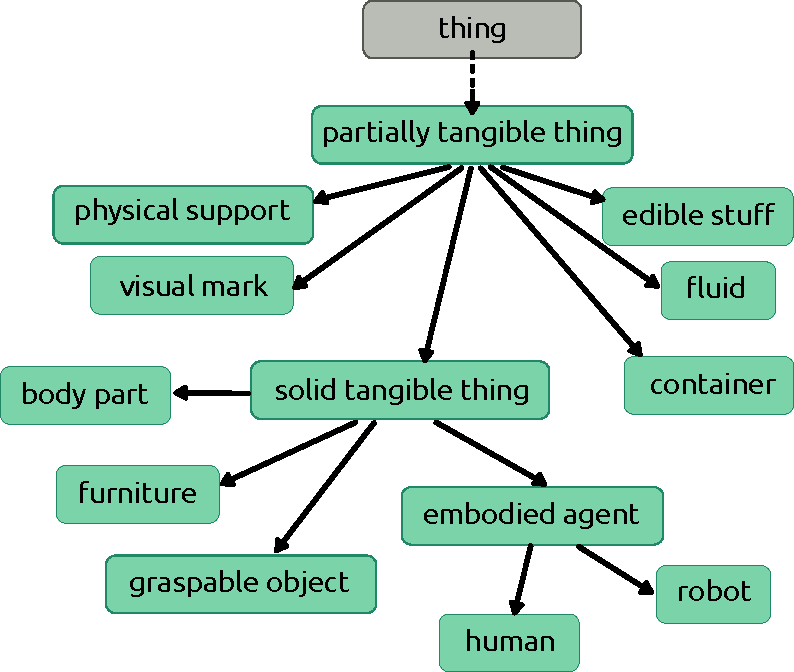
\includegraphics[width=0.6\columnwidth]{tangible_things_tbox.pdf}
    \caption{TBox of the specialisations of \concept{PartiallyTangible}.}
    \label{fig|tangible_things_tbox}
\end{figure}

This excerpt from the ontology makes the bottom-up design process visible: only
few types of \emph{partially tangible} things appear, and only subclasses
relevant to the context of service robotics in an human-like environment are
present. For performances and ease of use, we do not attempt to comprehensively
cover the field. We opportunistically extend the common-sense knowledge when
required by experiments.

Lastly, the ORO common-sense ontology contains several rules and class
expressions that encode non-trivial inferences.

The definition of the \concept{Bottle} is a case in point:

\concept{Bottle} $\equiv$ \concept{Container} {\bf and} \concept{Tableware}
{\bf that} (\concept{hasShape} {\bf value} \concept{cylinderShape} {\bf and}
\concept{hasCharacteristicDimension} {\bf only} \concept{\em int[>= 0.1, <=
0.3]})

If a human informs the robot that a given object is indeed a bottle, the robot
can then infer much more on this object. And if the human affirms that a car is
a bottle, the robot may question this assertion because of the inconsistent
size.

We discuss in section~\ref{krs-discussion} the strengths and weaknesses of our
knowledge framework.

\subsection{Internal cognitive processes}
\label{sect|intern}

\subsubsection{Theory of Mind}
\label{sect|tom}

Theory of Mind (originally defined in~\cite{Premack1978}) is the cognitive
ability that a subject possesses to represent the mental state of another
agent, possibly including knowledge that contradicts the subject's own model: for
example, a book can be at the same time \emph{visible} for myself, and \emph{not
visible} for you.

Children develop this skill, which is essential to understand others' perspectives during
interactions, around the age of three. It supposes the
ability to build, store and retrieve separate models of the knowledge of the
interactors.

Our knowledge base implements such a mechanism: when the robots infers a new
agent has been introduced in the knowledge base, it initializes a new,
independent, ontology for this agent. All the ontologies that are created share
the same common-sense knowledge, but rely on each agent's perspective for the
actual instantiation: the robot (geometrically) computes that the book is in
its own field of view, but not in the human one. The robot knowledge contains
the fact \stmt{book isVisible true} while the human model contains \stmt{book
isVisible false}.

One classical application of this cognitive skill is the so-called
\emph{False-Belief} experiment (also known as the \emph{Sally and Ann}
experiment)~\cite{Leslie2000}: a child is asked to watch a scene where two
people, A and B, manipulate objects. Then A leaves and B hides away one
object. When A comes back, we ask the child ``where do you think A will
look for the object?''. Before acquiring a theory of mind, children are not
able to separate their own (true) model of the world (where they know that
the object was hidden) from the model of A, which contains \emph{false
beliefs} on the world (A still thinks the object is at its original
position since he did not see B hiding it). Using separate knowledge models
in the knowledge base, we have been able to replicate this experience with
our robots~\cite{warnier2012when}.

\subsubsection{Working memory}

The {\sc Oro} server also features a mechanism to mimic minimalistic forms of
memory families.  When new statements are inserted in the knowledge base, a
\emph{memory profile} is optionally attached to them.

Three such profiles are predefined: {\tt short term}, {\tt episodic} and {\tt
long term}. They are currently attached to different lifetime for the statements
(respectively 10 seconds, 5 minutes and no time limit). After this duration,
the statements are automatically removed from the knowledge base.

This approach is limited. In particular, \emph{episodic} memory should primarily
refer to the semantics of the statements (that is expected to be related to an
event) and not to a specific life duration.

We rely however on this mechanism in certain cases: for instance, some modules
like the natural language processor use the {\tt short term} memory profile to
mark for a few seconds important concepts that are currently manipulated by the
robot as \emph{active concepts}. For example, if a human asks the robot: ``Give
me all red objects'', the human, the \concept{Give} action, and each red
objects that are found are successively marked as \emph{active concepts} by
inserting statements such as \stmt{human type ActiveConcept} in the short-term
memory (which can be considered, in this case, to be a working memory). We use
this feature to trace certain knowledge-related processes.


%%%%%%%%%%%%%%%%%%%%%%%%%%%%%%%%%%%%%%%%%%%%%%%%%%%%%%%%%%%%%%%%%%%%%%%%%%%%%%%%
\section{Implementing the Cognitive Skills}
\label{sec:impl}

Previous section provided an overview of our cognitive architecture for robots
involved in interactions with other social agents, as well as the knowledge
model we rely on.

We now introduce each of the components and give insights on their main
features.


\subsection{Situation Assessment, Human Awareness, Perspective Taking}
\label{sect|sit-ass}

\begin{figure}
        \centering
        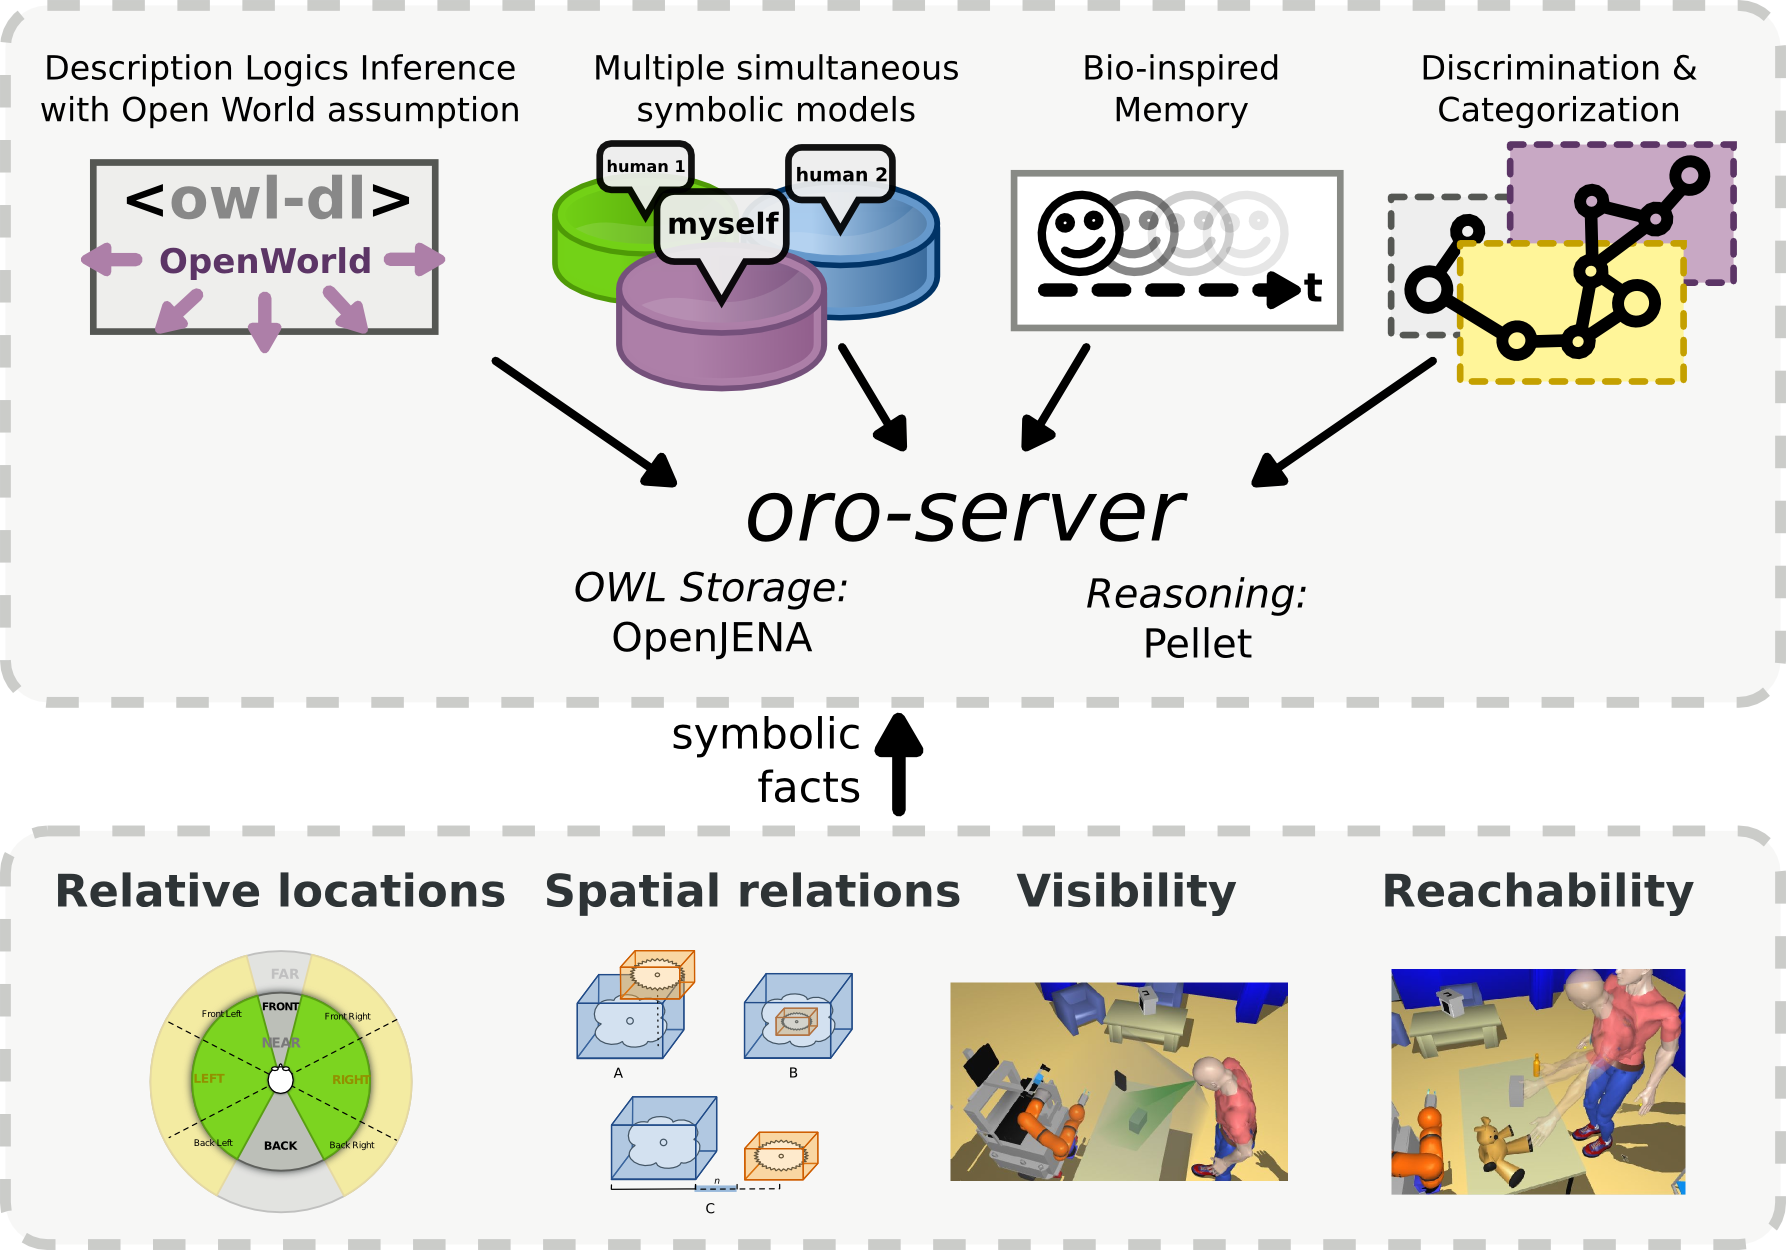
\includegraphics[width=\columnwidth]{spark-oro.png}
    \caption{Functional overview of knowledge base ({\sc Oro} server, top part)
    and the geometric situation assessment module (\emph{{\sc Spark}}, bottom
    part). {\sc Spark} computes symbolic relationships between objects and
    agents, and feeds them to the knowledge base.}

        \label{fig|spark-oro}
\end{figure}

Anchoring perceptions in a symbolic model requires perception abilities and
their symbolic interpretation. We rely on a dedicated geometric and temporal
reasoning module called {\sc Spark} (\emph{SPAtial Reasoning \&
Knowledge}~\cite{Sisbot2011}). It is a situation assessment reasoner that
generates symbolic knowledge from the geometry of the environment with respect
to relations between objects, robots and humans (Figures~\ref{fig|spark-oro} and~\ref{fig:sparkSubfigures}),
also taking into account the different perspective that each agent has on the
environment.

{\sc Spark} is an \emph{amodal}~\cite{Mavridis2006} geometric model of the
environment that serves both as basis for the fusion of the perception
modalities and as bridge with the symbolic layer. This geometric model is
continuously updated at run-time by the robot based on its sensors (in our
experiments, objects are identified and localised through 2D fiducial markers, while
humans are tracked with Kinect-like devices, optionally assisted by motion
capture to accurately track the head motion, which is required to compute what
the human is looking at).

From an artificial intelligence perspective, {\sc Spark} takes care of merging
sensing modalities, it computes and grounds perceptions into symbolic
knowledge (situation assessment), it is responsible temporal interpretation of
situations and performs spatial perspective-taking.

\begin{figure*}[ht!]
   \begin{center}
%
       \subfigure[Initial state]{%
%           \label{fig:wuweiPhoto}
           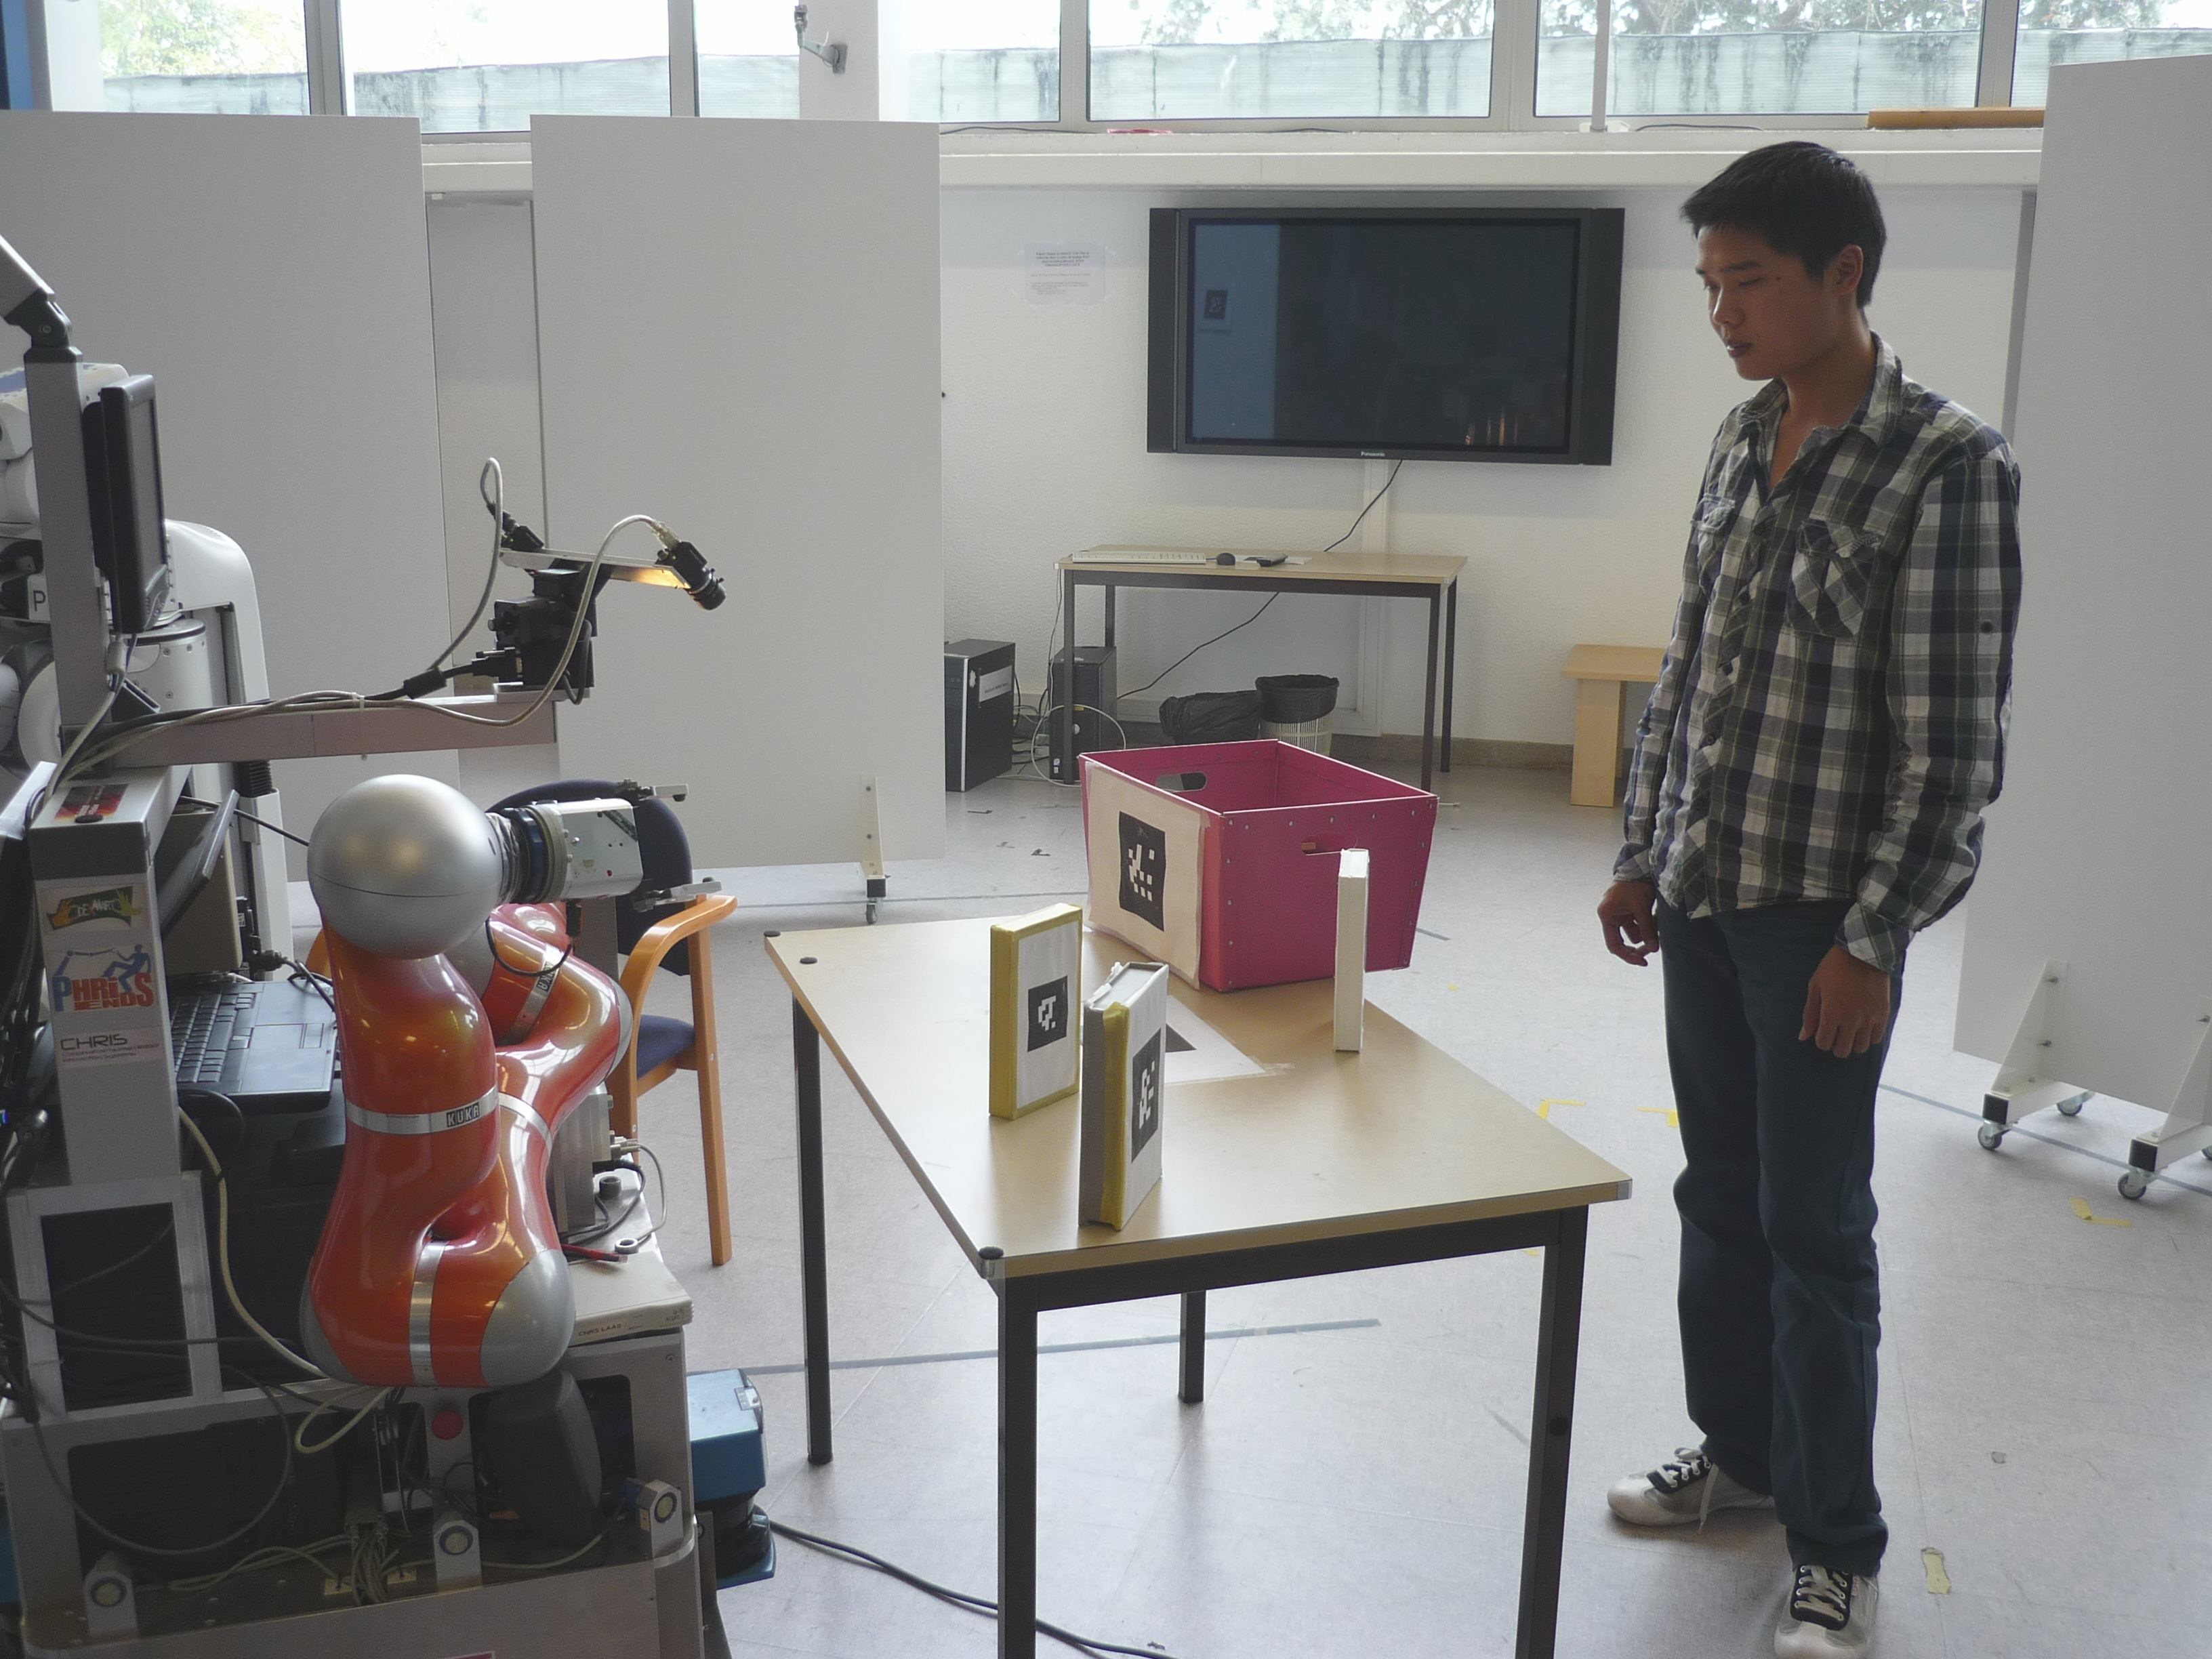
\includegraphics[width=0.5\textwidth]{etat2-P1010769_brightened-v2.jpg}
       }%
       \subfigure[Corresponding 3D model view]{%
%          \label{fig:sparkScreenshot}
          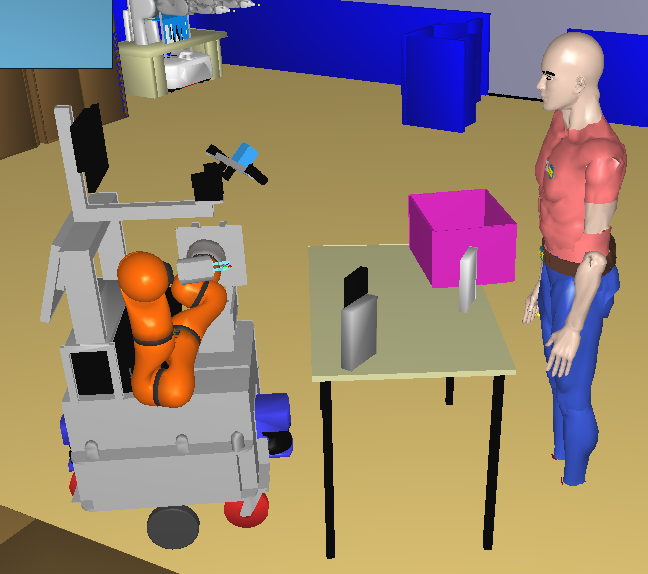
\includegraphics[width=0.43\textwidth]{etat2_photo.png}
       }\\ %  ------- End of the first row ----------------------%
%
   \end{center}

   \caption{% In this situation, there are three tapes on the table. Two tapes
       are only reachable by the robot: the \concept{LOTR\_TAPE} (black in the 3D
       model) and \concept{GREY\_TAPE}. The third tape \concept{WALLE\_TAPE} (white
       in the 3D model) and the trashbin \concept{PINK\_TRASHBIN} are only
       reachable by the human \concept{HUMAN1}. All tapes are on the table
   \concept{TABLE}. The corresponding symbolic facts are listed in Table~\ref{table|beliefsfig7}.  }%
 
 \label{fig:sparkSubfigures}

\end{figure*}

\begin{table}
\begin{center}
\begin{tabular}{l}
\hline
Robot's beliefs about itself (\emph{robot's model}):\\
\hline
  \hspace{0.7cm}\stmt{PINK\_TRASHBIN isReachable false}\\
  \hspace{0.7cm}\stmt{WALLE\_TAPE isReachable {\bf false}}\\
  \hspace{0.7cm}\stmt{LOTR\_TAPE isReachable {\bf true}}\\
  \hspace{0.7cm}\stmt{GREY\_TAPE isReachable {\bf true}}\\
  \hspace{0.7cm}\stmt{WALLE\_TAPE isVisible true}\\
  \hspace{0.7cm}\stmt{LOTR\_TAPE isVisible true}\\
  \hspace{0.7cm}\stmt{GREY\_TAPE isVisible true}\\
  \hspace{0.7cm}\stmt{WALLE\_TAPE isOn TABLE}\\
  \hspace{0.7cm}\stmt{LOTR\_TAPE isOn TABLE}\\
  \hspace{0.7cm}\stmt{GREY\_TAPE isOn TABLE}\\
\hline
\hline
Robot's beliefs about the human (\emph{human's model}):\\
\hline
  \hspace{0.7cm}\stmt{PINK\_TRASHBIN isReachable false}\\
  \hspace{0.7cm}\stmt{WALLE\_TAPE isReachable {\bf true}}\\
      \hspace{0.7cm}\stmt{LOTR\_TAPE isReachable {\bf false}}\\
      \hspace{0.7cm}\stmt{GREY\_TAPE isReachable {\bf false}}\\
  \hspace{0.7cm}\stmt{WALLE\_TAPE isVisible true}\\
  \hspace{0.7cm}\stmt{LOTR\_TAPE isVisible true}\\
  \hspace{0.7cm}\stmt{GREY\_TAPE isVisible true}\\
  \hspace{0.7cm}\stmt{WALLE\_TAPE isOn TABLE}\\
  \hspace{0.7cm}\stmt{LOTR\_TAPE isOn TABLE}\\
  \hspace{0.7cm}\stmt{GREY\_TAPE isOn TABLE}\\ 
 \hline
\end{tabular}
\end{center}
\caption{Symbolic facts computed from the situation depicted in
Figure~\ref{fig:sparkSubfigures}. Note how reachability differs for the two
agents.}

\label{table|beliefsfig7}
\end{table}

\subsubsection{Situation Assessment}

\paragraph{Symbolic facts production} 

Geometric state of the world is abstracted in symbolic facts that can
be classified in three different categories.

\begin {itemize}
\item Relative positions of object and agents, e.g.  \stmt{GREY\_TAPE
    isOn TABLE}.

\item Perception and manipulation capacity and state of agents,
  e.g. \stmt{ROBOT looksAt GREY\_TAPE}, \stmt{GREY\_TAPE isVisibleBy
    HUMAN1}.

\item Motion status for object or agent parts, e.g.  \stmt{GREY\_TAPE
    isMoving true},\\ \stmt{ROBOT\_HEAD isTurning true}.
\end {itemize} 

Reasoning about human perspective allow to compute facts such as:
\stmt{GREY\_TAPE isBehind HUMAN1}, \stmt{GREY\_TAPE leftOf
  HUMAN1}.

Figure~\ref{fig::reach-ex} illustrates different situations for the
\textit{reachable} relation.

\begin{figure*}[!t]
	\centering
    \subfigure[] { 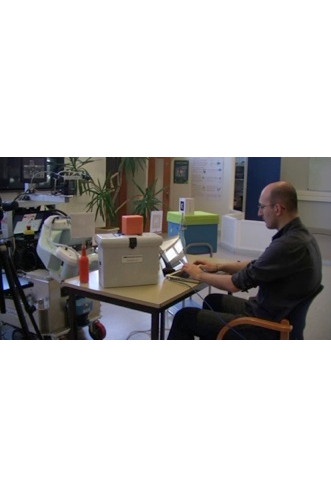
\includegraphics[width=0.2\textwidth]{reachex-1.png} }
    \subfigure[] {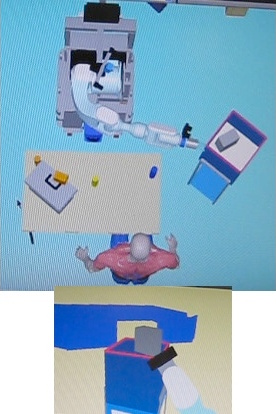
\includegraphics[width=0.2\textwidth]{reachex-2.jpg} }
    \subfigure[] {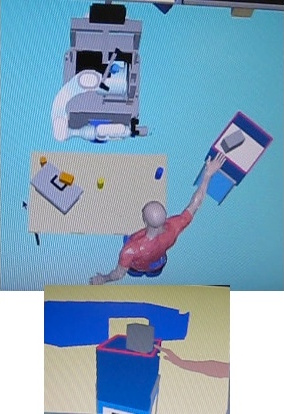
\includegraphics[width=0.2\textwidth]{reachex-3.jpg} }
    \subfigure[] {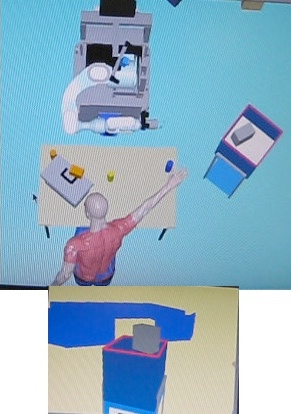
\includegraphics[width=0.2\textwidth]{reachex-4.jpg} }
    \caption{An example illustrating the \textit{reachable} relation. The
        relation is computed from the perspectives of both the robot and the
        human. The computed posture at each step is illustrated with a global
        view of the scene (top), and from a closest view (bottom). The robot
        and its human partner are placed face to face (a).  The robot first
        estimates if the small grey box is reachable to itself. This is done by
        finding a collision free posture to reach the object (b). Next the
        robot switches to the human's perspective to estimate if the same
        object is reachable to the human as well (c).  In the last scene, the
        human moves towards his left, farther from the object (d). The
        situation is then reevaluated. In this occasion though, the reasoner
        cannot find a satisfactory posture for the human to reach the box
        because he is too far from the target.  }

\label{fig::reach-ex}
\end{figure*}


\paragraph{Hypotheses on objects states and positions}
It is sometimes difficult or even impossible to see and/or track an
object in certain states. This happens, for instance, when the object
is hidden in a container, when the robot holds it in its gripper, and more
generally in any state in which it is hidden by something else. {\sc Spark} models the possible symbolic states of objects (whether the object is on a furniture, in an agent hand,
in a container, etc.): According to the robot perception of what has
happened since the object was last seen, the robot builds a
belief of the current possible state with associated probability for the.

\paragraph{Primitive action recognition} Monitoring human activity is crucial
to maintain a coherent state of the world. Full human action and activity
monitoring is a task that requires knowledge and reasoning both on high level
facts like goals, intentions and plans, as well as bottom-up data from agent
and object motions. Simple temporal and geometric reasoning on human hand
trajectories and potential objects placements can provide some useful clues for
high level human monitoring processes. We call this temporal and geometric
reasoning \emph{primitive action recognition}. Those primitive actions are
assessed through monitoring situations like ``an empty hand is close to an
object on a table'' (precursor for a \emph{pick}), or ``a hand holding an
object is over a container'' (precursor for a \emph{throw}).

\subsubsection{Ego-centric and allo-centric frames}

{\sc Spark} also supports \emph{perspective-taking}: spatial relations between entities can
be computed from different viewpoints, which let the robot build for each
agents it interacts with a different, \emph{perspective-aware} symbolic model
of the environment. These models are separately stored in the knowledge base.

This allows us to deal with ambiguities that arise when one speaker refers to
an object within a reference system (or changes the reference system, \ie
switches perspective) without making the reference frame
explicit~\cite{Breazeal2006, Ros2010}.

As a result, the robot stores models of the environment either in the
\emph{ego-centric} reference frame (from the robot perspective) or in 
\emph{allo-centric} frames (addressee-centred).

%%%%%%%%%%%%%%%%%%%%%%%%%%%%%%%%%%%%%%%%%%%%%%%%%%%%%%%%%%%%%%%%%%%%%%%%%%%%%%%%
\subsection{Multi-modal Communication}
\label{sect|com}

\subsubsection{Natural language grounding}

Natural language processing is one of the fields of human-robot interaction
for which the introduction of the semantic layer has been most beneficial.
In~\cite{Lemaignan2011a} we detail the techniques and the tool called
\texttt{dialogs} that we have developed for natural English language parsing and
grounding, along with verbalisation and (minimalist) dialogue management.

Natural language input (in experiments, we rely on an Android-based interface,
with Google speech recognition) is parsed into a grammatical structure, and
atoms of each sentence are resolved with the help of the ontology to ground
concepts like objects (\ie when a user says ``pick the can'', it resolves to which
instance of \emph{can} the user is referring to) and actions. Sentences are
sorted into questions, desires and statements, and processed accordingly.
Figure~\ref{dialogs|ex} gives a example of the processing of a simple order.

\begin{figure}
    \centering
	\begin{tabular}{l|l}
	\emph{Initial human knowledge} &
	\emph{Human input}\\
	
	\hline
	
    	\stmt{book\_1 type Book} &
	``Give me the book.'' \\
	
    	\stmt{book\_1 hasColor blue} & \\
	\vspace{0.5em}\\
	\hline
    	
	\emph{Generated partial statements} &
	\emph{Newly created statements}\\
	\hline
    	\stmt{?obj type Book} & 
	\stmt{human desires sit\_1} \\
	
	\hspace{0.2cm}$\Rightarrow$ \concept{?obj = book\_1}
    	& \stmt{sit\_1 type Give} \\
    	& \stmt{sit\_1 performedBy myself} \\
    	& \stmt{sit\_1 actsOnObject book\_01} \\
    	& \stmt{sit\_1 receivedBy human} \\
	\end{tabular}

    \caption{Processing an order: this simple example (no ambiguity), taken
    from~\cite{Lemaignan2011a}, shows the thematic roles computed by {\sc
Dialogs} for the order ``Give me the book''.}

\label{dialogs|ex}
\end{figure}


The system supports quantification (``give me \{a | the | some | all | any |
...\} can''), thematic roles (action-specific predicates that qualify the
actions), interactive disambiguation (the robot asks questions when it needs
more information), anaphora resolution (``give \emph{it} to me'') based on
dialogue history. It also permits knowledge extension by learning new semantic
structures (for instance, a sentence like ``learn that cats are animals'' is
converted into \stmt{Cat subClassOf Animal} and added to the knowledge base),
interprets common temporal and place adverbs (like \emph{above} or
\emph{tomorrow}) and translates to a certain extend \emph{states} (``I'm
tired'') into \emph{experiences} (\stmt{HUMAN experiences state\_1, state\_1
hasFeature tired}).

\subsubsection{Multi-modal communication}

Because all components rely on the same RDF formalism to format their outputs,
the different communication modalities (\emph{explicit} like verbal, deictic or
based on gaze, or \emph{implicit} like postures) are presented in a homogeneous
way, as statements in the knowledge base. The dialogue grounding process makes
use of them at two distinct levels to provide seamless multi-modal interaction.

First, particular steps of the grounding process explicitly check for the
presence and value of specific facts: for instance, when several instances
matches a category (the human says ``give me the bottle'' and the robot knows
about three bottles), the module may decide (it actually depends on the
quantifier preceding the class) to discard some of them based on their
\emph{visibility} for the speaker (implicit communication context built on the
human posture).

Another example, when the human says ``this'', the robot checks if the human is
currently pointing at some object. In that case, \emph{this} is replaced by the
object focused on.

Note that, while the system benefits from the complementary modalities, they
are not all required. The dialogue system can run with only the verbal
modality, at the cost of a simpler interaction.

The second level of integration of multi-modality is implicit: by computing
symbolic properties from the geometry, richer descriptions and hence
discrimination possibilities are available: for instance, if reachability is
available, the robot may ask ``do you mean the bottle that is accessible to
me?'' to discriminate between the three bottles. That way, procedures relying
on discrimination transparently benefit from added modalities.

%%%%%%%%%%%%%%%%%%%%%%%%%%%%%%%%%%%%%%%%%%%%%%%%%%%%%%%%%%%%%%%%%%%%%%%%%%%%%%%%

\subsection{Human-aware task planning}

Our execution controllers rely on symbolic task planning to convert long-term
desires into a succession of atomic actions. We use in our architecture the
HATP planner (for Human Aware Task Planner~\cite{Alili2008, Alili2009}).  HATP
is a refinement of a Hierarchical Task Network (HTN). As an HTN, it performs an
iterative task decomposition into sub-tasks until reaching atomic actions. The
\emph{planning domain} defines the set of methods describing how to decompose a
task and represents the procedural knowledge of the robot. It is stored outside
of the central knowledge base, using a specific formalism.

HATP originality resides in its ability to produce plans for the robot's
actions \emph{as well as for the other participants} (humans or robots): the
robot plans for itself, but also for its interactors, which effectively endows the robot
with new interaction capabilities: It can partially predict the behaviour, and
thus monitor the engagement, of its human partner; the planner generates
synchronisation points (arrow going from the robot stream to the human stream on
Figure~\ref{plan_hatp1}) between the agents; the controller can also verbalize
the plans to explain its partner how a task may be shared~\cite{warnier2012when}.

HATP can be tuned by setting up different costs depending on the actions to
apply and by taking into account a set of constraints called \emph{social
rules}. This tuning aims at adapting the robot's behavior according to the
desired level of cooperation of the robot.

\paragraph{Agents and action streams}
The robot plans not only for itself but also for the other agents. The
resulting plan, called ``shared plan'' is a set of actions that form
a stream for each agent involved in the goal achievement. Depending on
the context, some ``shared plans'' contain causal relations between
agents. For example, the second agent needs to wait for the success of
the first agent's action to be able to start its own action. When the
plan is performed, causal links induce synchronization between
agents. Figure~\ref{plan_hatp1} illustrates a plan with two streams.

\begin{figure}[htbp]
  \centering
  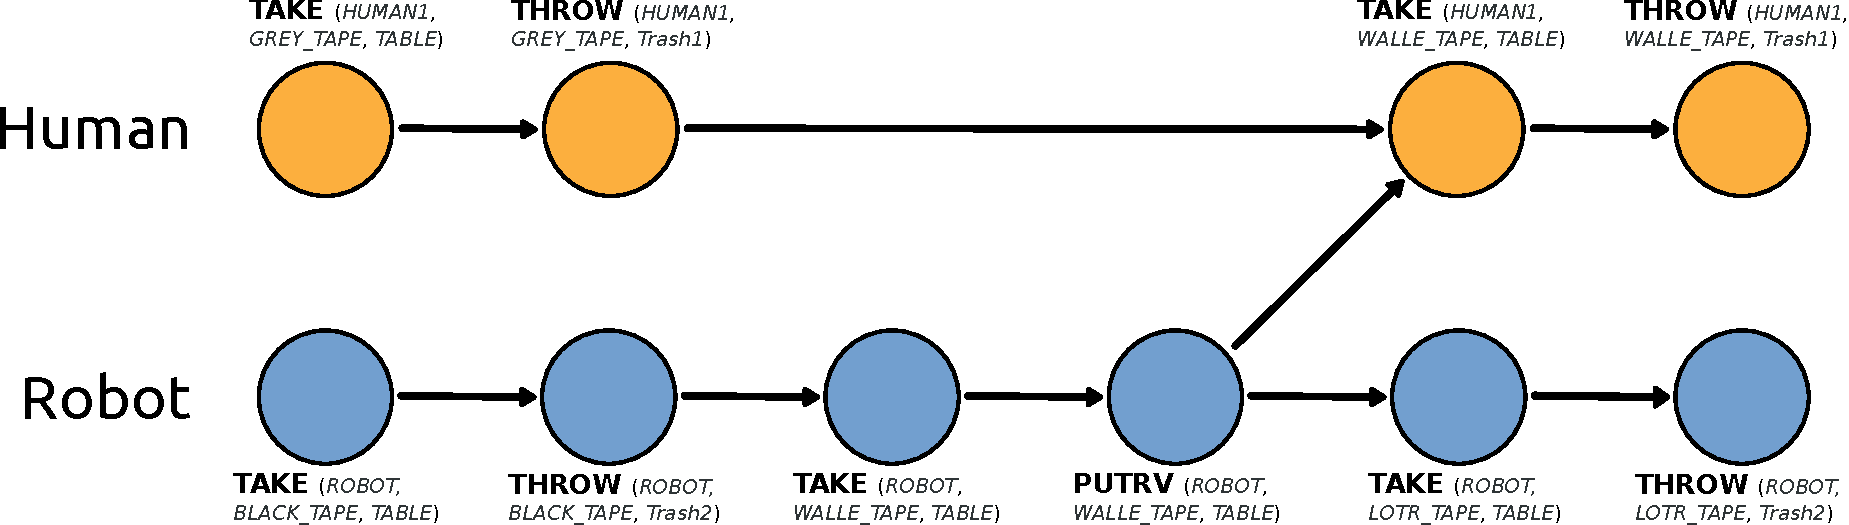
\includegraphics[width=0.95\columnwidth]{first_plan.pdf}
  \caption{A plan produced by HATP with 2 streams}
  \label{plan_hatp1}
\end{figure}

\paragraph{Action costs and social rules}
A cost and a duration function is associated to each action.
The duration function provides a duration interval for the action
achievement and is used, in one hand, to schedule the different
streams and, in the other hand, as an additional cost function.
In addition to these costs, HATP also takes into account a set of social
rules.  Social rules are constraints aiming at leading the plan
construction towards the best plan according to some human
preferences. The social rules we have defined so far deal with:

\begin{itemize}
\item undesirable state: to avoid a state in which the human could
  feel uncomfortable;
\item undesirable sequence: to eliminate sequences of actions that can
  be misinterpreted by the human;
\item effort balancing: to adjust the work effort of the agents;
\item wasted time: used to avoid long delays between the actions of
  the human partner;
\item intricate links: to limit dependencies between the actions of
  two or more agents.
\end{itemize}

\begin{figure}[htbp]
  \centering
  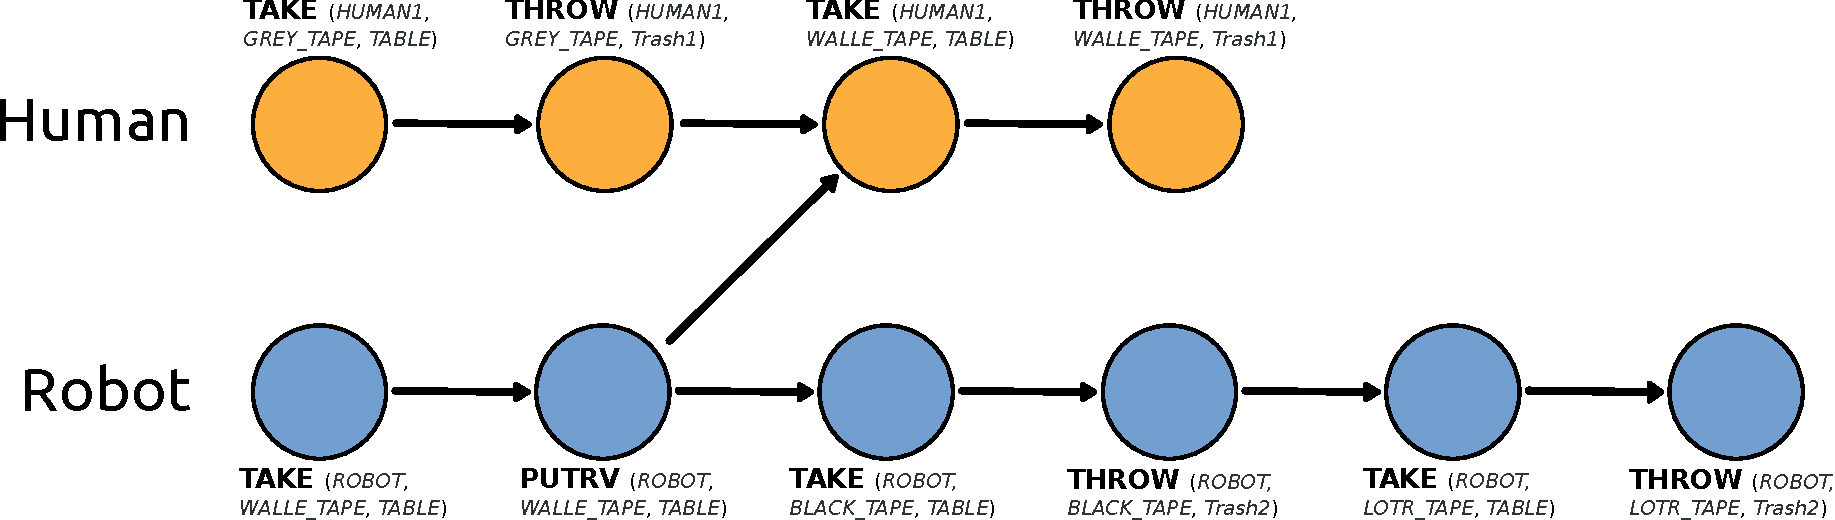
\includegraphics[width=0.95\columnwidth]{second_plan.pdf}
  \caption{A plan with the wasted time social rule. {\tt PUTRV} stands for {\it Put it so it is both Reachable and Visible}.}
  \label{plan_hatp2}
\end{figure}

Figure~\ref{plan_hatp2} illustrates an alternative plan to the previous 
one (Figure~\ref{plan_hatp1}) if the wasted time social rule is used.
The obtained shared plan is the best plan according to a global evaluation of
these multiple criteria.

\paragraph{Several levels of cooperation} 
By tuning its costs
and adapting its social rules, HATP can be used to compute various
alternative plans. These plans can be categorized into several levels
of cooperation

\begin{itemize}
\item helping the human to achieve his goal by acting for him
\item sharing concrete resources by handing some objects
\item collaboration of the robot and the human by coordinating their
  actions towards a human-robot joint goal.
\end{itemize}



Two important remarks: because HATP is a generic symbolic task planner, we have
been able to design a planning domain at a semantic level which is close to the
one used in the human-robot dialogue (the planner vocabulary contains concepts
like \texttt{give}, \texttt{table}, \texttt{is on}...). Hence only a few
ontology rules have been required to map both the knowledge extracted from the
situation assessment and the statements originated from the verbal interaction
to the planner domain.

Second remark, after some research (see appendix B of~\cite{Lemaignan2012a} for
a detailed discussion)  we have decided to represent neither the planning
domain nor the resulting plans in the knowledge base: the planning domain (with
task pre- and postconditions) is stored in a specific format, outside of the
central declarative knowledge repository, and the plans are directly
communicated to the robot controller. Thus, like many other cognitive
architectures, we have independent declarative and procedural knowledge stores.


%%%%%%%%%%%%%%%%%%%%%%%%%%%%%%%%%%%%%%%%%%%%%%%%%%%%%%%%%%%%%%%%%%%%%%%%%%%%%%%%
\subsection{Robot control}
\label{sect|ctrl}

\subsubsection{Desires and experiences}

Our robot execution controllers (OpenPRS-based {\sc Shary} or Python-based {\sc
pyRobots}) rely on extensive integration with the knowledge base. It serves as the
primary source of information for semantic-aware decision-making.

We split the interaction situations stemming from the situation assessment and
communication components in two categories: \emph{desires} (performative act)
and \emph{experiences} (assertive act).

\emph{Desires} are typically human orders (``Give me that book''). The nature
of the desired action (to pick, give, look, bring, show...), along with the
action parametrization (what is acted on? who should perform the action? etc.)
are extracted from the knowledge base, and either passed to a task planner
(presented in the previous section) or executed if the procedure is directly
available.

\emph{Experiences}, on the other hand, comprise of emotions, states and
questions (when asking a question, we consider the human to be in an
\emph{interrogative state}). When the knowledge base states that an agent
\emph{experiences} a particular emotion or state, the execution controller may
decide to handle it, typically by trying to answer the question or using the
emotional or physical state as a parameter for subsequent actions. As an
example, when the speaker says ``I feel tired'', we change the motion planner
parametrization to lower the effort the human needs to provide for the
following joint manipulation tasks. Note that this example has been implemented
as a proof-of-concept. A broader framework that would support action alteration
based on the user's experienced states is yet to be devised.

\subsubsection{Event-driven control}

The {\sc Oro} server proposes two paradigms to access its content: RPC-style
queries (based on the standard SPARQL language) or events. A module can
subscribe to an event by passing through an event pattern (in its simplest
form, a partial statement like \stmt{? type Elephant}) and a callback.  Each
time a new instance of elephant appears in the knowledge base, the callback is
triggered.

This allows us to write reactive robot controllers with a high level of
expressiveness: for instance, by subscribing to the event \stmt{human1 desires
?action, ?action type Look, ?action hasGoal myself}, we could trigger a
behaviour when the human expresses (through dialogue, gestures...) that he
wants to look at the robot itself.

The robot controller designer does not need to directly care about how this
\emph{desire} is produced (this is delegated to perception modules), he can
focus on the semantic of the desire.

Note also that we take advantage of the reasoning capabilities of the system:
for example, the goal of the action (\stmt{action hasGoal myself}) may not be
explicitly asserted, but inferred by the reasoner based on other assertions.

\subsubsection{Action execution and monitoring}\label{sec:action}

Action execution and monitoring is the central activity of the robot executive
controller, and involves interaction with most of the components presented on
Figure~\ref{fig|archi}.

Like most robotic architecture, actions are split into \emph{atomic actions}
and more complex \emph{tasks}. Tasks are created either statically or dynamically.
The {\sc pyRobots} controller, for instance, combines the actions listed in
table~\ref{table|pyrobots_actions} to implement the high-level tasks it exposes: {\tt
lookAt}, {\tt moveTo}, {\tt getFromHuman}, {\tt showObject}, {\tt giveObject},
{\tt pickObject}, {\tt bringObject}, {\tt putObject}, {\tt hideObject}.

Our other controller, {\sc Shary}, relies on the symbolic task planner to
generate at runtime suitable sets of atomic actions.

\begin{table}
\begin{center}
\begin{tabular}{p{8cm}}
\hline
    {\bf Manipulation} \\
     {\tt attachobject}, {\tt basicgive}, {\tt basictake}, {\tt close\_gripper}, {\tt configure\_grippers}, {\tt grab\_gripper}, {\tt handover}, {\tt hide}, {\tt open\_gripper}, {\tt pick}, {\tt put}, {\tt put\_accessible}, {\tt release\_gripper}, {\tt show}, {\tt take} \\
\hline
    {\bf Gaze control} \\
     {\tt glance\_to}, {\tt look\_at}, {\tt sweep}, {\tt switch\_active\_stereo\_pair}, {\tt track}, {\tt cancel\_track} \\
\hline
    {\bf Navigation} \\
     {\tt carry}, {\tt follow}, {\tt cancel\_follow}, {\tt goto}, {\tt moveclose}, {\tt waypoints} \\
\hline
    {\bf Local navigation} \\
     {\tt dock}, {\tt rotate}, {\tt translate} \\
\hline
    {\bf Posture configuration} \\
     {\tt extractpose}, {\tt idle}, {\tt manipose}, {\tt movearm}, {\tt rest}, {\tt setpose}, {\tt settorso}, {\tt tuckedpose} \\
\hline
\end{tabular}
\end{center}
\caption{Main {\sc pyRobots} \emph{actions}, sorted by categories. These
actions are combined at runtime into higher-level \emph{tasks}.}

\label{table|pyrobots_actions}
\end{table}

\paragraph{Human aware motion, placement and manipulation planning}
Manipulation and navigation actions listed in
table~\ref{table|pyrobots_actions} rely on a collection of dedicated 3D motion
planner to generate movements that are aware of surrounding humans. Robot
placement and end-effectors trajectories are computed on-line to allow object
manipulation that take into account task specific constraints and human
postures, abilities and preferences. \cite{Sisbot2008, Mainprice2011,
Pandey2011} detail these techniques.


\paragraph{Action Execution and Monitoring Robot Controller}
Based on context and on the shared plan elaborated by HATP for a given goal,
the robot controller decides to execute an action or to ask its human
partner to do it.  Actions feasibility by the human or the robot are
regularly reconsidered based on the reachability / visibility
computation mechanisms.

Robot action execution is based on simple automatons  that translate
symbolic planning atomic actions into sequences of planned arm motions
and gripper commands to execute according to current state
of the 3-tuple (gripper, object, furniture). We have three states
according to whether the object is in gripper and if it is in gripper
whether it is on furniture.  These states are directly obtained from
the updated symbolic state of the world in the ontology.

For plan action monitoring, primitive actions recognition is used. A primitive
action detection is interpreted as action success if it is the expected one and
failure otherwise. The robot also reacts to the absence of activity.



%%%%%%%%%%%%%%%%%%%%%%%%%%%%%%%%%%%%%%%%%%%%%%%%%%%%%%%%%%%%%%%%%%%%%%%%%%%%%%%%
%%%%%%%%%%%%%%%%%%%%%%%%%%%%%%%%%%%%%%%%%%%%%%%%%%%%%%%%%%%%%%%%%%%%%%%%%%%%%%%%
%%%%%%%%%%%%%%%%%%%%%%%%%%%%%%%%%%%%%%%%%%%%%%%%%%%%%%%%%%%%%%%%%%%%%%%%%%%%%%%%

\section{Experimental outcomes}
\label{sec:expe}

Our architecture has been deployed and tested in a number of experiments on
several robotic platforms. Table~\ref{table|experiences} lists the most
significant ones, with their main focuses and reference publications for the
interested reader.

\begin{table*}
\begin{center}

\begin{tabular}{llll}
 \bf{Experiment} & Focus & \emph{Notes} & Reference \\
\hline
{\it Point \& Learn} (2010) & Interactive knowledge acquisition & & \cite{Lemaignan2010} \\
{\it Spy Game} (2010) & Interactive object discrimination & & \cite{Ros2010b} \\
{\it Moving to London} (2011) & Multi-modal interaction, perspective taking & \emph{immobile robot} & \cite{lemaignan2011what} \\
{\it Roboscopie} (2011) & Theater, reflection on the future of HRI & \emph{semi-autonomous} & \cite{lemaignan2012roboscopie} \\
{\it Cleaning the table} (2011) & Full integration & & \cite{Alami2011} \\
{\it I'm in your shoes} (2012) & False beliefs & & \cite{warnier2012when} \\
{\it Give me this} (2012) & Natural joint object manipulation & & \cite{gharbi2013natural} \\
{\it Aperitif time} (2012) & Multi-modal interaction, perspective taking & & \cite{lemaignan2013talking} \\
\hline

\end{tabular}
\end{center}
\caption{Main experiments conducted with our cognitive architecture.}
\label{table|experiences}
\end{table*}

The two following sections present one such experiment (the {\it Moving to
London} scenario), and the synopsis of another one (the {\it Cleaning the
table} scenario).

The first one is focused on knowledge representation and verbal interaction:
the human asks for help to find and pack objects. In this experiment, robot
actions are limited to simple motions (like head tracking or predefined
pick-and-place).

The second one involves the SHARY execution controller and the HATP symbolic
task planner besides ORO and {\sc Dialogs}. In this scenario, the human and the
robot try to cooperatively remove objects from a table. Behaviours and motions
are fully planned.

\subsection{\emph{Moving to London} scenario}

This first experiment is based on the following daily life situation: Tom and
Jerry are moving to London, so they are packing things in boxes. The scenario
takes places in the living-room, where Jido (our robot) is observing while they
move things here and there. To assess the reasoning abilities of the robot they
ask Jido for information. Ideally, the robot should
also perform actions when required (\eg hand an object when asking ``give
me...'').

Perception of objects is done through a tag-based system and humans are
detected through motion capture. The robot knowledge base is pre-loaded with
the \emph{ORO Commonsense Ontology}.  We next describe two
situations where we can follow the internal robot's reasoning and the
interaction with the users.

\paragraph{Implicit disambiguation through visual perspective taking}

\begin{figure}[!ht]
  \centering
  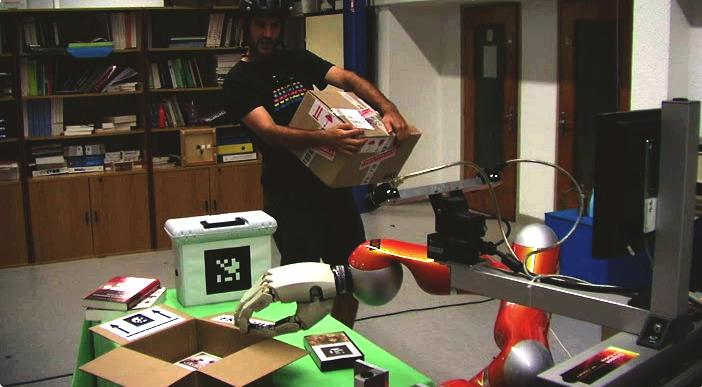
\includegraphics[width=0.9\linewidth]{pt.jpg}
\caption{Asking the robot to hand over a tape on the table.}
  \label{fig|vpt}
\end{figure}


Tom enters the room while carrying a big box (Figure~\ref{fig|vpt}). He
approaches the table and asks Jido to hand him the video tape: ``Jido, can
you give me the video tape''. The \textsc{Dialogs} module queries the ontology to
identify the object the human is referring to: \stmt{?obj type VideoTape}. 

There are two video tapes in the scene: one on the table, and another one
inside the cardboard box. Thus, the knowledge base returns both: $\Rightarrow$
\concept{?obj = [videoTape1, videoTape2]}. 

However, only one is visible for Tom (the one on the
table). Thus, although there is an ambiguity from the robot's perspective
(since it can see both video tapes), based on the perspective of its human
partner it infers that Tom is referring to the video tape on the table, and not
the one inside the box which is not visible for him.

Since only one object remains, the robot infers
that the human refers to it and would eventually execute the command, \ie give
it to the human. Alternatively, the robot could first verify with the human if
that was the object being referred to or not before proceeding to execute the
action. Table~\ref{table|ptbeliefs} lists the robot's beliefs about itself and
its human partner involved in this situation.

\begin{table}
\begin{center}
\begin{tabular}{l}
\hline
Robot's beliefs about itself (\emph{robot's model}):\\
\hline
  \hspace{0.7cm}\stmt{videoTape1 type VideoTape}\\
  \hspace{0.7cm}\stmt{videoTape1 isOn table}\\
  \hspace{0.7cm}\stmt{videoTape1 isVisible true}\\
  \hspace{0.7cm}\stmt{videoTape2 type VideoTape}\\
  \hspace{0.7cm}\stmt{videoTape2 isIn cardBoardBox}\\
  \hspace{0.7cm}\stmt{videoTape2 isVisible true}\\
\hline
\hline
Robot's beliefs about Tom (\emph{Tom's model}):\\
\hline
  \hspace{0.7cm}\stmt{videoTape1 type VideoTape}\\
  \hspace{0.7cm}\stmt{videoTape1 isOn table}\\
  \hspace{0.7cm}\stmt{videoTape1 isVisible true}\\
  \hspace{0.7cm}\stmt{videoTape2 type VideoTape}\\
  \hspace{0.7cm}\stmt{videoTape2 isIn cardBoardBox}\\
  \hspace{0.7cm}\stmt{videoTape2 isVisible false}\\
 \hline
\end{tabular}
\end{center}
\caption{Robot's beliefs about itself and its human partner.}
\label{table|ptbeliefs}
\end{table}

\paragraph{Explicit disambiguation through verbal interaction and gestures}

\begin{figure}[!ht]
  \centering
  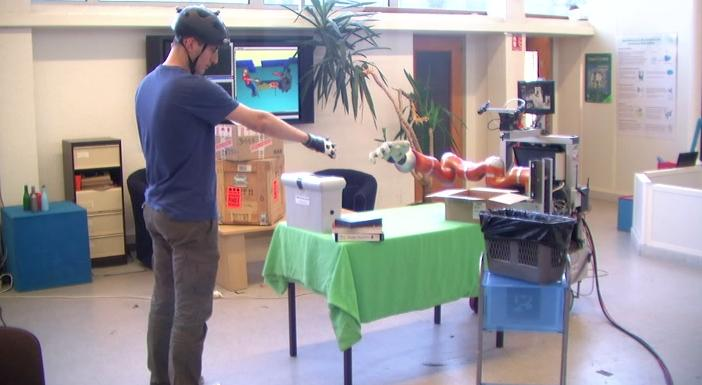
\includegraphics[width=0.9\linewidth]{inTheBox2.jpg}
\caption{Jerry asks Jido for the content of the box by pointing at it.}
  \label{fig|pointing}
\end{figure}

In this situation, Jerry enters the living room without knowing where Tom had
placed the video tapes (Figure~\ref{fig|pointing}). So he first asks Jido:
``What's in the box?''. Before the robot can answer the question it has to
figure out which box Jerry is talking about. Similar to the previous situation,
there are two available boxes: 

\begin{center}
\begin{tabular}{l}
\stmt{?obj type box}\\
\hspace{0.7cm}$\Rightarrow$ {\tt ?obj = [cardBoardBox, toolbox]}
\end{tabular}
\end{center}

However both are visible and the cognitive ambiguity resolution cannot be
applied. The only option is to ask Jerry which box he is referring to: ``Which
box, the toolbox or the cardboard box?'' Jerry could answer the
question. Instead, he decides to point at it while indicating: ``This box''
(Figure~\ref{fig|pointing}). The robot's perception identifies the {\tt
cardBoardBox} as being pointed at and looked at by the human and updates the
ontology with this new information using a rule available in the commonsense
ontology ({\tt \textbf{pointsAt}(?ag, ?obj) $\land$ \textbf{looksAt}(?ag, ?obj) $\to$
\textbf{focusesOn}(?ag, ?obj)}) The \textsc{Dialogs} module is then able to merge both
sources of information, verbal (``this'') and deictic to distinguish the box
Jerry refers to.

\begin{center}
\begin{tabular}{l}
\stmt{Jerry pointsAt carboardBox}\\
\stmt{Jerry looksAt carboardBox}\\
$\to$ \stmt{Jerry focusesAt carboardBox}\\
\hspace{0.7cm}$\Rightarrow$ {\tt ?obj = [cardBoardBox]}
\end{tabular}
\end{center}

Finally, the \textsc{Dialogs} queries the ontology about the content of the box
and the question can be answered: ``Jido-E''. Note that the object's label is
used instead of its ID. This way we enhance interaction using familiar names
given by the users.

\begin{center}
\begin{tabular}{l}
\stmt{?obj isIn cardBoardBox}\\
\hspace{0.7cm}$\Rightarrow$ \concept{?obj = videoTape2}\\
\end{tabular}
\end{center}

At this point Jerry wants to know where the other tape is, and that is exactly
what he asks Jido: ``And where is the other tape?''. In this situation, the
\textsc{Dialogs} module is able to interpret that Jerry is not referring to the
video which they were just talking about, but to the other one:

\begin{center}
\begin{tabular}{l}
\stmt{?obj type VideoTape}\\
\stmt{?obj differentFrom videoTape2}\\
\hspace{0.7cm}$\Rightarrow$ \concept{?obj = [videoTape1]}
\end{tabular}
\end{center}

Since there is only one possible ``other'' video (there are only two videos in
the scene), it can directly answer Jerry: ``The other tape is on the table and
next to the toolbox.''

\begin{center}
\begin{tabular}{l}
\stmt{videoTape1 isOn table}\\
\stmt{videoTape1 isNextTo toolbox}
\end{tabular}
\end{center}


\subsection{\emph{Cleaning the table} scenario}

This experiment involved a more complex decisional layer where the ORO server
was used in conjunction with the HATP symbolic task planner and the SHARY
execution controller (the complete software architecture we deployed for this
experiment is the one pictured on Figure~\ref{fig|archi},
page~\pageref{fig|archi}).

In this scenario (Figure~\ref{fig|cleantable-video}), a human and a robot
cooperate to remove objects from a table. The robot produces symbolic plans for
both itself and the human (Figure~\ref{plan-etat2})
that allow the robot to (verbally) share the task with the human (like ``I take
the green box and I put it in the trashbin, you take the black video tape and
you throw it in the trashbin''). Plans are created based on perceived
visibility and reachability of the objects, and the robot also monitors the
human activities to track the advancement of the whole plan.

\begin{figure}
    \centering
    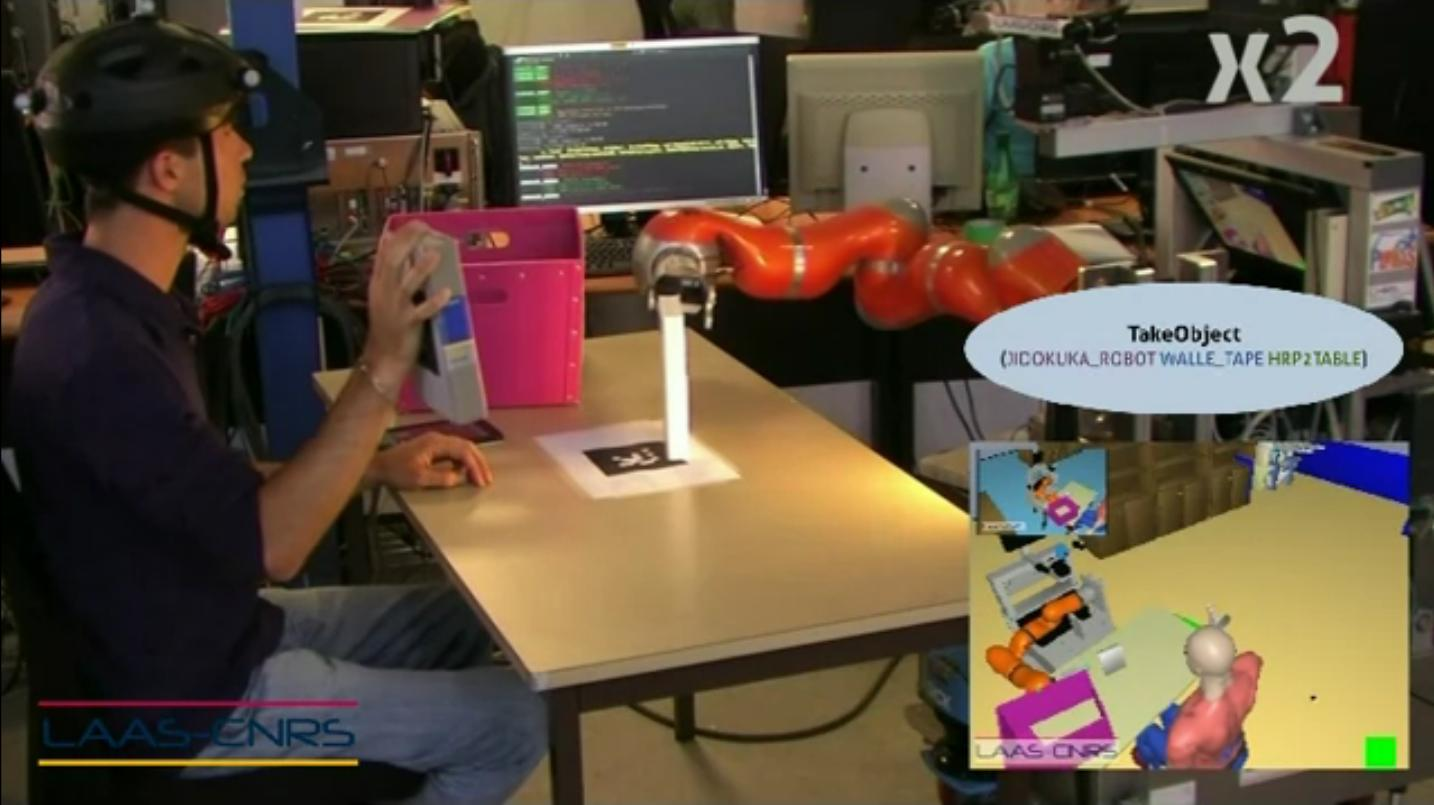
\includegraphics[width=0.7\columnwidth]{cleantable.jpg}

    \caption{Snapshot of the film of the ``Clean the Table'' scenario. The
    physical situation, the {\sc Spark} model, and the current step of the plan can
    be seen.}

    \label{fig|cleantable-video}
\end{figure}

\begin{figure*}[thpb]
  \centering
  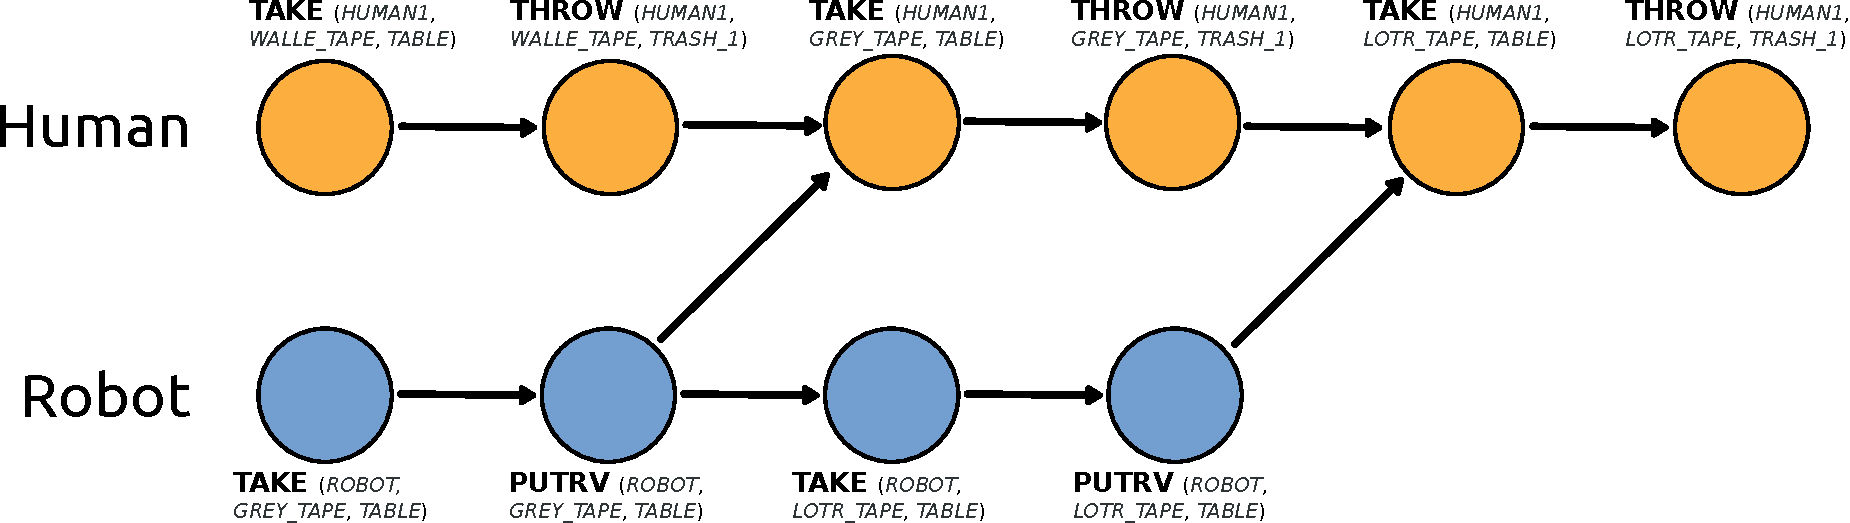
\includegraphics[width=1.0\textwidth]{third_plan.pdf} \\
  \caption {A plan produced by HATP to execute the high-level order ``clean the table''. Two streams of actions are generated: for the human (top) and for the robot(bottom). Synchronization points ensure the coordination.}
  \label{plan-etat2}
\end{figure*}

Figure~\ref{fig|cleantable-timeline} presents a sample of the whole task and
shows how the different components produce and use symbolic knowledge.

This sequence of events depicts a run with only one tape on the table. The tape is
reachable by the robot only, while the human is the one who can reach the
trashbin to throw objects.

\begin{figure*}[thpb]
  \centering
    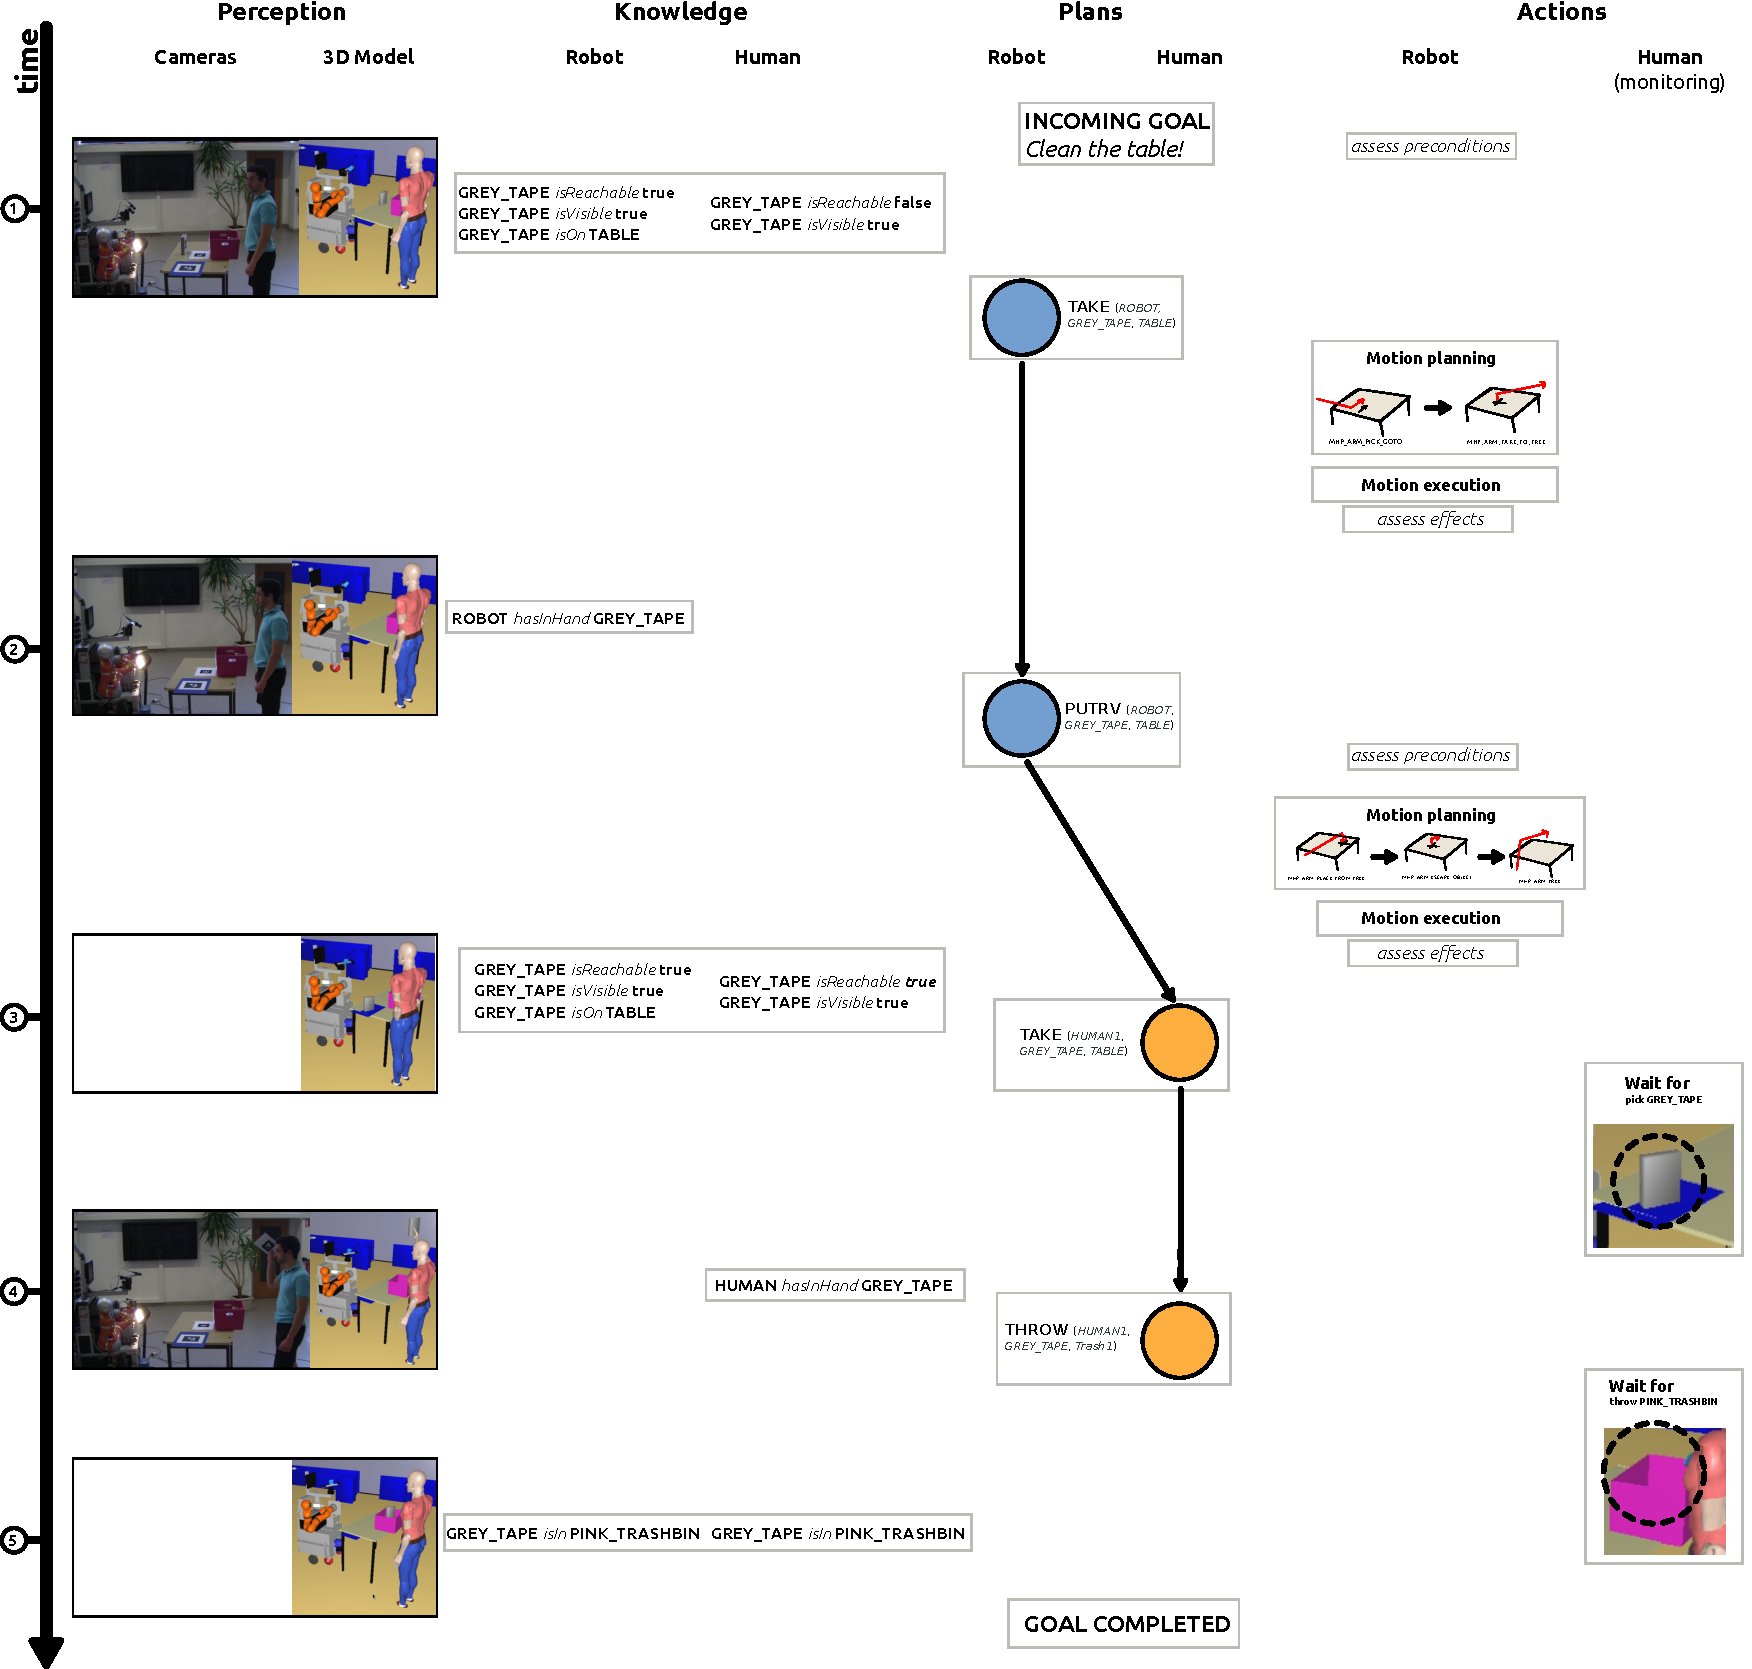
\includegraphics[width=1.0\textwidth]{manip_run.pdf} \\
        \caption {Sequence of events of a simplified version of the \emph{Cleaning the table} scenario.}
  \label{fig|cleantable-timeline}
\end{figure*}


The plan produced in that case by HATP is straightforward and shown in the
third row. It consists in four successive actions involving the robot and the
human. Robot grasps the tape and then places it on the table at a position
where it is visible and reachable for the human. Human then is asked to pick
the tape and throw it in the trashbin.

%%%%%%%%%%%%%%%%%%%%%%%%%%%%%%%%%%%%%%%%%%%%%%%%%%%%%%%%%%%%%%%%%%%%%%%%%%%%%%%%
%%%%%%%%%%%%%%%%%%%%%%%%%%%%%%%%%%%%%%%%%%%%%%%%%%%%%%%%%%%%%%%%%%%%%%%%%%%%%%%%
%%%%%%%%%%%%%%%%%%%%%%%%%%%%%%%%%%%%%%%%%%%%%%%%%%%%%%%%%%%%%%%%%%%%%%%%%%%%%%%%

\section{Discussion: when AI enables HRI}
\label{sect|conclusion}

This last section goes over again the main contributions we have presented
so far: why they are relevant to robotics and artificial intelligence, how do
they compare to similar approaches, how do we support our technical choices and
what remains to be developed/explored in the future.

\subsection{Foundations of cognition for the robot}

Because we build autonomous \emph{companion} robots, designed to live and
interact in environments primarily conceived for humans, we endow our machines
with a set of fundamental cognitive capabilities. The robots perform typically
in dynamics, partially unknown environments, with a variety of places,
artifacts and agents that may carry complex semantics.

While our main focus is on the cognitive abilities required to interact with
humans, \emph{situation assessment}, \emph{spatial reasoning}, \emph{knowledge
representation and reasoning}, \emph{task planning} or \emph{high-level
control} are mandatory cognitive foundations to build upon.

\paragraph{Situation assessment, spatial reasoning}

Real service robots need to ground their decision-making processes in their
perceptions, be it physical (\eg what a camera sees) or not (\eg remote
knowledge bases, dialogue). We call \emph{physical situation assessment} the
cognitive skill that a robot exhibits when it assesses the nature and content of its
surroundings and efficiently monitors its evolution.

Numerous approaches exist, like amodal \emph{proxies}~\cite{Jacobsson2008},
grounded amodal representations~\cite{Mavridis2006}, semantic maps
(\cite{Nuechter2008, Galindo2008,Blodow2011}) or
affordance-based planing and object classification~\cite{Lorken2008,
Varadarajan2011}.

Our approach, implemented in the {\sc Spark} module, is a grounded amodal
representation of the robot environment, where different sensing modalities
(vision-based fiducial markers tracking, RGBD human tracking, motion capture)
are merged and where amodal spatial reasoning takes place (for instance,
explanation generation for unexpected perceptions like a disappearing object).

Spatial reasoning~\cite{O'Keefe1999} is a field in its own right, and has been
used for natural language processing for applications such as direction
recognition ~\cite{Kollar2010,Matuszek2010} or language
grounding~\cite{Tellex2010}.~\cite{Skubic2004} present a spatial reasoner
integrated in a robot which computes symbolic positions of objects.

One of the main limit of our current approach is the way semantics are
conveyed: because we use 2D markers for artifacts, we skip most of the object
extraction and recognition challenges. Each object has a unique identifier,
which enable us to load a proper CAD model suitable for 3D spatial reasoning
and prevent recognition mistakes in the knowledge base. While {\sc Spark}
algorithms themselves are ignorant of the input sources, and would work equally
well with a full object recognition stack, we have not tackled it yet.

Besides, temporal reasoning (essential for accurate action recognition for
instance) is not properly addressed in our stack. Temporal reasoning is used
only locally, and does not allow for tracking of long or global events.

\paragraph{Robot control}

\fxwarning{Robot control related work -> what is the originality of SHARY? why is it relevant from an AI point of view? (Mathieu, Aurelie)}

Beetz et al.~\cite{Beetz2010} proposes a cognitive architecture called
\textsc{CRAM} (Cognitive Robot Abstract Machine) that integrates
\textsc{KnowRob}~\cite{Tenorth2009a}, a knowledge processing framework based on
Prolog. Its underlying storage is based on an OWL ontology, derived from
\textsc{OpenCyc}. \textsc{CRAM} and \textsc{KnowRob} have been demonstrated on
several real-world scenarios, where natural language recipes extracted from the
Internet had to be translated into plans and executed in a kitchen environment,
perceived and rebuilt on-line by the robots.

\fxwarning{robot control architecture for service robots: what else?}

\subsection{Knowledge framework}
\label{krs-discussion}

Knowledge flows in our architecture through a \emph{semantic blackboard}, the
{\sc Oro}-server. We rely on Description Logics (OWL) to represent and
manipulate facts.

Relying on RDF triples and Description Logics has advantages such as good
understanding of its trades-off, thanks to being widespread in the semantic Web
community, the availability of mature libraries to manipulate the ontology,
interoperability with several major on-line knowledge bases ({\sc
OpenCyc}, {\sc WordNet}, {\sc DBPedia} or {\sc RoboEarth}~\cite{Waibel2011} are
some examples), open-world reasoning, and the formal guarantee of decidability
(it is always possible to classify a Description Logics ontology).

It also has notable limitations, both fundamental (the suitability of
Description Logics when reasoning on --typically non-monotonic-- commonsense
knowledge is questionable) and practical: RDF triples imply only binary
predicates, which constrains the expressiveness of the system or leads to
cumbersome reifications. Alternatives exist (like {\sc
KnowRob}~\cite{Tenorth2009a}) that mix RDF with more expressive logic languages
like {\sc Prolog}, at the price, however, of other limitations, like
closed-world reasoning or immutable T-Box. The classification performance is
another issue: from our experience, with an ontology sized for a standard
experiment (about 100 classes and 200 instances), classification typically
takes about 100ms, which becomes problematic during interactions.  Besides, the
performances are difficult to predict, since a seemingly inoffensive new
statement may indirectly change abruptly the logical complexity of the whole
knowledge model and lead to notable degradation of classification time.

This knowledge model also largely excludes representation of continuous
phenomena (like time) or uncertain phenomena. When required (for instance for
action recognition), these are managed by dedicated components (like {\sc
Spark}), and are not exposed at the semantic level.

Tools to manipulate and reason over ontologies are readily available, mature,
and already well accepted in the robotic community~\cite{Tenorth2009a,
Lim2011}. Alternatives like \emph{Answer Set Programming} have also been
successfully investigated in robotics~\cite{Chen2010,Erdem2012}, in particular
to deal with non-monotonic reasoning. However we did not actually hit any brick wall
while working with OWL ontologies. We may reconsider this choice at a later
stage, but until now it has proven an effective framework to quickly explore
implementations of new cognitive abilities (for instance, it has been
conceptually and technically easy to add support for independent knowledge
models, one per agent the robot interacts with --see section~\ref{sect|tom}).

Besides, because ontologies and RDF statements are relatively simple concepts
to grasp, it also effectively helped to grow awareness amongst colleagues on
the significance of the ``semantic level'' when developing new components for
the robot.

\subsection{Interacting with humans}

\paragraph{Building a model of a human during the interaction} Perspective
Taking is a human ability which allows one to put him/herself in another
person's point of view. Studied in psychology
literature~\cite{Flavell1992,Tversky1999}, this ability is crucial when
interacting with people by allowing one to reason on others' understanding of
the world in terms of visual perception, spatial descriptions, affordances and
beliefs, etc.  In the last years these notions have been gradually
employed in HRI.~\cite{Breazeal2006} presents a learning
algorithm that takes into account information about a teacher's visual
perspective in order to learn a task. ~\cite{Johnson2005} apply visual
perspective taking for action recognition between two
robots.~\cite{Trafton2005} use both visual and spatial perspective taking to
find out the referent indicated by a human partner.

\fxwarning{What are our contribution regarding perspective taking? (Mathieu)}
\fxwarning{Mention other source of knowledge about humans -- including social rules for instance}

\paragraph{Reasoning with the humans}

\fxwarning{Mention we represent the human knowledge as well (Severin)}

\paragraph{Limits of disambiguation at semantic level}

\fxwarning{Introduce the paragraph} 

One prototypical example of semantic disambiguation has been given in
\cite{Ros2010b} with the child game \emph{spygame}: two players are facing
each other with a set of random objects in-between, one player mentally choose
one object, and the other player has to guess the object by asking closed
questions like \emph{Is your object small or large?} Based on the knowledge it
has acquired, the robot is able to minimize the number of questions required to
find the object.

When playing this kind of game, however, the issue arises that the robot has no
way to select which knowledge about the object is relevant in the interaction
context. For instance, the knowledge base may store facts like \stmt{obj1 type
ActiveConcept} (which internally means that this concept was mentioned in a
discussion in the last few seconds): this information is not a relevant
property of \concept{obj1} when trying to disambiguate concepts with humans.
This distinction between \emph{internal knowledge} (meaningful to
the system only) and \emph{common knowledge} (whose meaning is understood by
all the interactors) has not been properly dealt with in our architecture.

Besides, even knowledge that belongs to the \emph{common knowledge} may not be
appropriate in a given interaction context. For instance, the system may
compute that at a given instant the human is looking at the object: \stmt{human
looksAt obj1}. This property makes sense to both parties, but in the context of
the \emph{spygame}, we would like to mainly use immanent properties, not
volatile like a gaze. More research is required to identify relevant
interaction contexts and knowledge classes attached to them.

\subsection{Joint actions with humans}
\label{sec:soa}

The human presence brings new requirements for robot's abilities both
at the functional and at the deliberative levels~\cite{Klein2004}. The
topics involve motion~\cite{Kulic2007,Berg2004,Madhava2006},
navigation~\cite{Althaus2004,Sisbot2007}, manipulation~\cite{Kemp2007}
in presence of humans as well as perception of human
activities~\cite{Breazeal2001,Burger2008}. Also, when
interacting with humans, robots need to incorporate communication and
collaboration abilities. Several theories dealing with
collaboration~\cite{Cohen1991,Grosz1996,Clark1996} emphasize that
collaborative tasks have specific requirements compared to individual
ones, \eg, since the robot and the person share a common goal, they
have to agree on the manner to realize it, they must show their
commitment to the goal during execution, etc. Several robotic systems
have already been built based on these
theories~\cite{Rich1997,Sidner2005,Breazeal2003} and they
all have shown benefits of this approach. They have also shown how
difficult it is to manage turn-taking between communication partners
and to interleave task realization and communication in a generic
way. Finally, today only few
systems~\cite{Fong2006,Breazeal2003,Sisbot2008} take humans into
account at all levels.


\subsection{Knowledge-oriented architecture}

Altogether, the components we have presented compose a
\emph{knowledge-oriented} architecture:

\begin{itemize}
    
    \item{Knowledge is explicitly stored in one central and consistent
    repository of facts, accessible for all modules.} 

    \item{Knowledge is represented in a strict formalism (OWL statements) and
    with a clearly defined vocabulary (stated in the common-sense ontology).}

    \item{The first two points enable a loosely-coupled architecture where
    modules can be removed or replaced easily by other ones as long as
    they share the same semantics (modules are defined by the knowledge they
    produce),} 

    \item{We adopt a \emph{symbolic}, reactive, event-driven approach to robot control.
    By managing events at the same level as the reasoner, we take full
    advantage of the inference abilities of {\sc Oro} to trigger events whose
    \texttt{true} conditions can be inferred.} 

    \item{Finally, this architecture allows for the combination of very
    different knowledge modalities in a single homogeneous environment,
    bringing mutual benefits to components. For instance, the dialogue
    processing module can perfectly run without any geometric
    perception, but its disambiguation routines can transparently
    benefit from it when available (since richer symbolic descriptions of
    objects are then available).}

\end{itemize}

Those items are not new \emph{per se}. It is however interesting to
underline the shift of focus this implies during the design and integration
phases of robots: components of our deliberative layer are defined and glued together by
the knowledge they produce and consume.

It reveals how the robotic community is ``catching up'' with semantic
technologies. Human-robot interaction, because it supposes operations in
environments with complex semantics, drives this evolution.

\subsection{Embodied Cognition}

Robotics is traditionally regarded as the prototypical instance of \emph{embodied}
artificial intelligence, and this dimension is especially prevalent in
human-robot interaction, where agents have to share a joint physical
environment.

It results in a tight coupling between the symbolic and the geometric realms:
while AI at its origins was mostly a matter of symbolic models, it has been
since recognised that not only the mind is not a purely abstract system,
disconnected from the physical world, but even more, cognition fundamentally
relies on its relation to the physical world (so-called \emph{embodied
cognition}). Varela~\cite{Varela1992} is one of the main discoverer of these
mechanisms, and coined the concept of \emph{enactivism} as the theoretical
framework that study the links between cognition, embodiment and actions.

The challenge of symbol grounding is tightly linked to this issue. It
corresponds to the identification or creation, and then, maintenance of a link
between the symbol (the syntactic form of knowledge the computer will
manipulate) and its semantics, \ie its meaning, anchored in the world (the
relations between the symbol, the referent of the symbol, and mediating minds
is classically referred as the \emph{semantic triangle}, and has been
extensively studied in linguistics). The issue of grounding is well known in
cognitive science and is summarised by Harnard~\cite{Harnad1990} by this
question: ``how the semantic interpretation of a formal symbol system can be
made intrinsic to the system?''. This issue has a major practical importance in
robotic: for a robot to be both endowed with a symbolic representational and
reasoning system, and able to \emph{act} in the physical world, it must ground
its knowledge.

Grounding is implemented at different levels in our architecture. The main source
of grounded symbolic knowledge is the situation assessment module, {\sc Spark}.
Not only it builds symbolic facts from spatial reasoning, but it also relies on
temporal reasoning to track the world state and build explanations to interpret
unexpected perceptions (we mentioned above the example of a disappearing
object).

Because {\sc Spark} is also able to track humans, which enables in turn
perspective-aware spatial reasoning, it produces grounded symbolic knowledge
for interacting agents as well. This is a typical \emph{embodied} cognitive
skill.

Grounding also occurs during verbal and non-verbal communication. The {\sc
Dialogs} module grounds new concepts introduced by the speaker by asking questions
until it can attach the new concept to concepts already present in the
knowledge pool (typically, if I ask the robot ``bring me a platypus'', the
robot asks ``what is a platypus''. I may answer ``a mammal'' and the robot will
ask ``what is a mammal?'' and so on until it anchors the new concepts to ones
it already knows). Non verbal interaction (like gestures) is also partially
grounded. When the user points at something, it can say ``give me this'' and
the robot grounds \emph{this} to the pointed artifact.

Because only objects marked with tags are currently recognized (in our typical
lab experiments, it may be a dozen of them), the robot grounding mechanisms work
in a small-sized closed world. This assumption obviously greatly facilitates
the task. It remains to be seen if systematic marking of manipulated objects
(for instance with RFID tags) is a realistic path. It may be the case if the
robot is expected to be used in a well-defined, slowly changing environment.
Real-time recognition of large libraries of objects is another path which may
be viable soon~\cite{Dean2013Fast}.


\subsection{The Next Steps}

\fxwarning{Rewrite conclusion}

We have devised a decisional framework for human-robot interactive
task achievement that is aimed to allow the robot not only to
accomplish its tasks but also to produce behaviors that support its
engagement vis-a-vis its human partner and to interpret human
behaviors and intentions. 
Together and in coherence with this framework, we have developed
and experimented various task planners and interaction schemes that
allow the robot to select and perform its tasks while taking into
account explicitly the human abilities as well as the constraints
imposed by the presence of humans, their needs and preferences. 


In this paper we have presented a decisional framework designed for
robots operating in a human environment. Our objective is to provide a
management of human-robot interaction that is an integral part of a
general robot control architecture.  This was done in order to provide
a principled way to deal with HRI scenario.  The framework is also
suitable for the development and experiment of task planners and
interaction schemes that explicitly consider human abilities and
preferences.

The design choices and the results presented here are still preliminary.
While the general scheme we propose might be difficult to implement in
a general sense, we believe that it is a reasonable challenge to
implement it in the case of a personal robot assistant essentially
devoted to fetch-and-carry, as well as for interactive manipulation
tasks and associated activities.



\section*{Acknowledgments}

Building such a robotic architecture is the work of many hands, and we would
like to acknowledge here the worthwhile contributions of Samir Alili, Aurélie
Clodic, Raquel Ros Espinoza, Mamoun Gharbi, Julien Guitton, Matthieu Herrb, Jim
Mainprice and Amit Kumar Pandey.

This work has been supported by EU FP7 ``SAPHARI'' under grant agreement no.
ICT-287513.


\bibliographystyle{elsarticle-num}
%\bibliographystyle{abbrv}
\bibliography{laas_hri}



\end{document}
